%%%%%%%%%%%%%%%%%%%% LN-Book.tex %%%%%%%%%%%%%%%%%%%%%%%%%%%%%
%
% Stand: 2025/01/14 ulgr
%
%
%%%%%%%%%%%%%%%% Springer-Verlag %%%%%%%%%%%%%%%%%%%%%%%%%%


% RECOMMENDED %%%%%%%%%%%%%%%%%%%%%%%%%%%%%%%%%%%%%%%%%%%%%%%%%%%
\documentclass[graybox,envcountchap,sectrefs]{svmono}

% choose options for [] as required from the list
% in the Reference Guide

%\usepackage{mathptmx}
%\usepackage{helvet}
%\usepackage{courier}
%
\usepackage{type1cm}         

\usepackage{makeidx}         % allows index generation
\usepackage{graphicx}        % standard LaTeX graphics tool
                             % when including figure files
\usepackage{multicol}        % used for the two-column index
\usepackage[bottom]{footmisc}% places footnotes at page bottom

\usepackage{newtxtext}       % 
\usepackage[varvw]{newtxmath}       % selects Times Roman as basic font

% see the list of further useful packages
% in the Reference Guide
\usepackage[english]{babel}
\usepackage{csquotes}
\usepackage[inline,shortlabels]{enumitem}

%% -- Part A etc
%% -- A-I etc für \chapter
%% -- 1. für \section etc
%% --
\renewcommand\thepart{\Alph{part}}
%\renewcommand\thechapter{\thepart-\Roman{chapter}}
%\renewcommand\thesection{\arabic{section}}
%\renewcommand\thesubsection{\thesection.\arabic{subsection}}
%

%% -- Für Links im PDF
%% --
\usepackage{hyperref}
\hypersetup{%
	,breaklinks = true	%
	,colorlinks	= true  %  Farbige Links false/true, für onlineversion true                                                           
	,urlcolor	= blue  %                                                              
	,citecolor	= blue  %                                                          
	,linkcolor	= blue	% oder black
%  	,hidelinks 			% Vor dem Druck % entfernen
	}

%% -- \subsection nicht ins TOC
%% --
\setcounter{tocdepth}{1}

%% -- Durchgehende Nummerierung
%% -- siehe 
\makeatletter
\let\c@remark=\c@theorem 		% Make remark share the theorem counter
\let\c@definition=\c@theorem 	% Make definition share the theorem counter
\let\c@example=\c@theorem 		% Make example share the theorem counter
\let\c@lemma=\c@theorem 		% Make lemma share the theorem counter
\let\c@corollary=\c@theorem 	% Make corollary share the theorem counter
\let\c@proposition=\c@theorem 	% Make proposition share the theorem counter
\makeatother

%% --

\makeindex             % used for the subject index
                       % please use the style svind.ist with
                       % your makeindex program
                       
%% --

%%%%%%%%%%%%%%%%%%%%%%%%%%%%%%%%%%%%%%%%%%%%%%%%%%%%%%%%%%%%%%%%%%%%%

\date{Stand: \today}

\begin{document}

\author{Wolfgang Arendt, Annette Grabosch, G\"unther Greiner, Ulrich Groh, Heinrich P. Lotz, Ulrich Moustakas, Rainer Nagel, Frank Neubrander, Ulf Schlotterbeck}
%% --
\title{One-parameter Semigroups of Positive Operators\\
		{\large{Edited by R. Nagel}}}
%% --
\subtitle{Lecture Notes in Mathematics\\ \\ 1184\\ \\Springer-Verlag\\ Berlin Heidelberg New York Tokyo}
%% --
\maketitle

\frontmatter%%%%%%%%%%%%%%%%%%%%%%%%%%%%%%%%%%%%%%%%%%%%%%%%%%%%%%
%% -- part-0
% !TEX root = ../LN-Book.tex
%%%%%%%%%%%%%%%%%%%%%%% dedic.tex %%%%%%%%%%%%%%%%%%%%%%%%%%%%%%%%%
%
% dedication
% Stand: 2025/01/13 ulgr
% Use this file as a template for your own input.
%
%%%%%%%%%%%%%%%%%%%%%%%% Springer %%%%%%%%%%%%%%%%%%%%%%%%%%

\begin{dedication}
{\RaggedRight\Large 
This second edition of \emph{One-Parameter Semigroups of Positive Operators} is dedicated to the memory 	of our 
co-authors, Heinrich P.~Lotz (1934--2010) and Ulf Schlotterbeck (1941--2021). 
Their contributions to the first edition remain an inspiration to us all. 
We miss their presence and remain grateful for the legacy they have left in this work.}
\end{dedication}





%%%%%%%%%%%%%%%%%%%%%%%foreword.tex%%%%%%%%%%%%%%%%%%%%%%%%%%%%%%%%%
% sample foreword
%
% Use this file as a template for your own input.
%
%%%%%%%%%%%%%%%%%%%%%%%% Springer %%%%%%%%%%%%%%%%%%%%%%%%%%

\foreword

%% Please have the foreword written here
Use the template \textit{foreword.tex} together with the document class SVMono (monograph-type books) or SVMult (edited books) to style your foreword\index{foreword}. 

The foreword covers introductory remarks preceding the text of a book that are written by a \textit{person other than the author or editor} of the book. If applicable, the foreword precedes the preface which is written by the author or editor of the book.


\vspace{\baselineskip}
\begin{flushright}\noindent
Place, month year\hfill {\it Firstname  Surname}\\
\end{flushright}


% !TEX root = ../LN-Book.tex
%%%%%%%%%%%%%%%%%%%%%%preface.tex%%%%%%%%%%%%%%%%%%%%%%%%%%%%%%%%%%%%%%%%%
% preface
% 2025/03/17 ulgr
%
%%%%%%%%%%%%%%%%%%%%%%%% Springer %%%%%%%%%%%%%%%%%%%%%%%%%%

\preface

\section*{Preface to the Revised First Edition}
	
	When the first edition of these lecture notes appeared in 1986, the theory of one-parameter semigroups of positive operators was undergoing rapid development, stimulated by applications in ergodic theory, evolution equations, stochastics, and mathematical physics. 
	Our goal at the time was to provide a systematic and accessible account of the foundations and structure theory of positive semigroups, with particular emphasis on Banach lattices and \CA-algebras.
	We were gratified by the positive reception the volume received and the extent to which it found use in research and graduate instruction.
	
	Over the past four decades, the mathematical community has continued to draw on the results and techniques developed in these notes. 
	Despite the appearance of newer texts and the evolution of the field, this volume has remained widely cited and used—likely due to its thorough and methodical treatment of a core area in functional analysis. 
	The sustained interest from both researchers and students has encouraged us to prepare this revised first edition.
	
	We have preserved the structure and exposition of the original edition but have made a number of editorial improvements, including transferring the entire book into \LaTeX{}. 
	Obvious misprints have been corrected, references and the subject index have been updated where appropriate, and the notes at the end of each chapter have been expanded to some subsequent developments. 
	However, we have refrained from substantially altering the original content in order to retain the historical character and coherence of the text.
	
	We gratefully acknowledge the efforts of our co-author, Ulrich Groh, who guided the transfer of the manuscript into \LaTeX{}, with the assistance of Klaus-Georg Kuhn and the support of Claude, an artificial intelligence model developed by Anthropic.
	
	It is our hope that this revised edition will continue to serve as a valuable resource for those working in operator theory, functional analysis, and their many applications. 
	We remain deeply grateful to our colleagues and readers who have provided feedback and encouragement over the years.
%% --
%\begin{quote}
%{\itshape
%This second edition of \emph{One-Parameter Semigroups of Positive Operators} is dedicated to the memory 	of our 
%co-authors, Heinrich P.~Lotz (1934--2010) and Ulf Schlotterbeck (1941--2021). 
%Their contributions to the first edition remain an inspiration to us all. 
%We miss their presence and remain grateful for the legacy they have left in this work.}
%\end{quote}
%% --
%\vspace{.75em}
%{\RaggedLeft{The authors} }


%% Please write your preface here

\section*{Preface to the First Edition}

As early as 1948 in the first edition of his fundamental treatise on \emph{Semigroups and Functional Analysis}, E.~Hille expressed the need for 

\begin{quote}
\textit{\ldots developing an adequate theory of transformation semigroups operating in partially ordered spaces} (l.c., Foreword). 
\end{quote}

In the meantime the theory of one-parameter semigroups of positive linear operators has grown continuously. 
Motivated by problems in probability theory and partial differential equations W.~Feller (1952) and R.~S.~Phillips (1962) laid the first cornerstones by characterizing the generators of special positive semigroups. 
In the 60's and 70's the theory of positive operators on ordered Banach spaces was built systematically and is well documented in the monographs of H.~H.~Schaefer (1974) and A.~C.~Zaanen (1983). 
But in this process the original ties with the applications and, in particular, with initial value problems were at times obscured. 
Only in recent years an adequate and up-to-date theory emerged, largely based on the techniques developed for positive operators and thus recombining the functional analytic theory with the investigation of Cauchy problems having positive solutions to each positive initial value. 
Even though this development --- in particular with respect to applications to concrete evolution equations in transport theory, mathematical biology, and physics --- is far from being complete, the present volume is a first attempt to shape the multitude of available results into a coherent theory of one-parameter semigroups of positive linear operators on ordered Banach spaces.

The book is organized as follows.
We concentrate our attention on three subjects of semigroup theory: \emph{characterization}, \emph{spectral theory} and \emph{asymptotic behavior}. 
By \emph{characterization}, we understand the problem of describing special properties of a semigroup, such as positivity, through the generator. 
By \emph{spectral theory} we mean the investigation of the spectrum of a generator. 
\emph{Asymptotic behavior} refers to the orbits of the initial values under a given semigroup and phenomena such as stability.

This program (characterization, spectral theory, asymptotic behavior) is worked out on four different types of underlying spaces.
\newpage
%% --
\begin{enumerate}[label=(\Alph*)]
\item 
On Banach spaces---Here we present the background for the subsequent discussions related to order.

\item 
On spaces $C_{0}(X)$ ($X$ locally compact), which constitute an important class of ordered Banach spaces and where our results can be presented in a form which makes them accessible also for the non-expert in order-theory.

\item 
On Banach lattices, which admit a rich theory and are still sufficiently general as to include many concrete spaces appearing in analysis; e.g., $C_0(X)$, $\mathcal{L}^p(k)$ or $l^p$.

\item 
On non-commutative operator algebras such as \CA- or \WA-algebras, which are not lattice ordered but still possess an interesting order structure of great importance in mathematical physics.

\end{enumerate}
%% --
In each of these cases we start with a short collection of basic results and notations, so that the contents of the book may be visualized in the form of a $4 \times 4$ matrix in a way which will allow \enquote{row readers} (interested in semigroups on certain types of spaces) and \enquote{column readers} (interested in certain aspects) to find a path through the book corresponding to their interest.

We display this matrix, together with the names of the authors contributing to the subjects defined through this scheme.
%% --
%\definecolor{darkgreen}{rgb}{0.0, 0.75, 0.0}
%\begin{table}[ht]
%\centering
%\begin{tabular}{l|c|c|c|c|}
%\cline{2-5}
% & \color{darkgreen}{I} & II & \color{darkgreen}{III} & IV \\
% & \color{darkgreen}{Basic} & Characterization & \color{darkgreen}{Spectral} & Asymptotics \\
% & \color{darkgreen}{Results} &  & \color{darkgreen}{Theory} & \\
%\hline
%\multicolumn{1}{|l|}{A. Banach} & R. Nagel & W. Arendt & G. Greiner & F. Neubrander \\
%\multicolumn{1}{|l|}{Spaces} & U. Schlotterbeck & H. P. Lotz & R. Nagel & \\
%\hline
%\multicolumn{1}{|l|}{B. $C_0(X)$} & R. Nagel & W. Arendt & G. Greiner & A. Grabosch \\
%\multicolumn{1}{|l|}{} & U. Schlotterbeck & & & G. Greiner \\
%\multicolumn{1}{|l|}{} & & & & U. Moustakas \\
%\multicolumn{1}{|l|}{} & & & & F. Neubrander \\
%\hline
%\multicolumn{1}{|l|}{C. Banach} & R. Nagel & G. Arendt & G. Greiner & A. Grabosch \\
%\multicolumn{1}{|l|}{Lattices} & U. Schlotterbeck & & & G. Greiner \\
%\multicolumn{1}{|l|}{} & & & & U. Moustakas \\
%\multicolumn{1}{|l|}{} & & & & R. Nagel \\
%\multicolumn{1}{|l|}{} & & & & F. Neubrander \\
%\hline
%\multicolumn{1}{|l|}{\color{darkgreen}{D. Operator}} & U. Groh & U. Groh & U. Groh & U. Groh \\
%\multicolumn{1}{|l|}{\color{darkgreen}{Algebras}} & & & & \\
%\hline
%\end{tabular}
%\end{table}
%% --
%\definecolor{darkgreen}{rgb}{0.0, 0.75, 0.0}
%\begin{table}[ht]
%\centering
%\begin{tabular}{l|c|c|c|c|}
%\cline{2-5}
% & I & II & III & IV \\
% & Basic & Characterization & Spectral & Asymptotics \\
% & Results &  & Theory & \\
%\hline
%\multicolumn{1}{|>{\columncolor{darkgreen}}l|}{A. Banach} & {R. Nagel} & W. Arendt & G. Greiner & F. Neubrander \\
%\multicolumn{1}{|>{\columncolor{darkgreen}}l|}{Spaces} & U. Schlotterbeck & H. P. Lotz & R. Nagel & \\
%\hline
%\multicolumn{1}{|>{\columncolor{darkgreen}}l|}{B. $C_0(X)$} & R. Nagel & W. Arendt & G. Greiner & A. Grabosch \\
%\multicolumn{1}{|>{\columncolor{darkgreen}}l|}{} & U. Schlotterbeck & & & G. Greiner \\
%\multicolumn{1}{|>{\columncolor{darkgreen}}l|}{} & & & & U. Moustakas \\
%\multicolumn{1}{|>{\columncolor{darkgreen}}l|}{} & & & & F. Neubrander \\
%\hline
%\multicolumn{1}{|>{\columncolor{darkgreen}}l|}{C. Banach} & R. Nagel & G. Arendt & G. Greiner & A. Grabosch \\
%\multicolumn{1}{|>{\columncolor{darkgreen}}l|}{Lattices} & U. Schlotterbeck & & & G. Greiner \\
%\multicolumn{1}{|>{\columncolor{darkgreen}}l|}{} & & & & U. Moustakas \\
%\multicolumn{1}{|>{\columncolor{darkgreen}}l|}{} & & & & R. Nagel \\
%\multicolumn{1}{|>{\columncolor{darkgreen}}l|}{} & & & & F. Neubrander \\
%\hline
%\rowcolor{darkgreen}
%\multicolumn{1}{|l|}{D. Operator} & U. Groh & U. Groh & U. Groh & U. Groh \\
%\rowcolor{darkgreen}
%\multicolumn{1}{|l|}{Algebras} & & & & \\
%\hline
%\end{tabular}
%\end{table}
%%  --

\definecolor{darkgreen}{rgb}{0.0, 0.75, 0.0}

\begin{table}[ht]
\centering
%\begin{tabular}{l|>{\columncolor{darkgreen}}c|c|>{\columncolor{darkgreen}}c|c|}
\begin{tabular}{l|c|c|c|c|}
\cline{2-5}
 & I & II & III & IV \\
 & Basic & Characterization & Spectral & Asymptotics \\
 & Results &  & Theory & \\
\hline
\multicolumn{1}{|l|}{A. Banach} & R. Nagel & W. Arendt & G. Greiner & F. Neubrander \\
\multicolumn{1}{|l|}{Spaces} & U. Schlotterbeck & H. P. Lotz & R. Nagel & \\
\hline
\multicolumn{1}{|l|}{B. $C_0(X)$} & R. Nagel & W. Arendt & G. Greiner & A. Grabosch \\
\multicolumn{1}{|l|}{} & U. Schlotterbeck & & & G. Greiner \\
\multicolumn{1}{|l|}{} & & & & U. Moustakas \\
\multicolumn{1}{|l|}{} & & & & F. Neubrander \\
\hline
\multicolumn{1}{|l|}{C. Banach} & R. Nagel & W. Arendt & G. Greiner & A. Grabosch \\
\multicolumn{1}{|l|}{Lattices} & U. Schlotterbeck & & & G. Greiner \\
\multicolumn{1}{|l|}{} & & & & U. Moustakas \\
\multicolumn{1}{|l|}{} & & & & R. Nagel \\
\multicolumn{1}{|l|}{} & & & & F. Neubrander \\
\hline
%\rowcolor{darkgreen}
\multicolumn{1}{|l|}{D. Operator} & U. Groh & U. Groh & U. Groh & U. Groh \\
%\rowcolor{darkgreen}
\multicolumn{1}{|l|}{Algebras} & & & & \\
\hline
\end{tabular}
\end{table}
%% --
This \enquote{matrix of contents} has been an indispensable guide line in our discussions on the scope and the spirit of the various contributions. 
However, we would not have succeeded in completing this manuscript, as a collection of independent contributions (personally accounted for by the authors), under less favorable conditions than we have actually met. 
For one thing, Rainer Nagel was an unfaltering and undisputed spiritus rector from the very beginning of the project. 
On the other hand we gratefully acknowledge the influence of Helmut H.~Schaefer and his pioneering work on order structures in analysis. 
It was the team spirit produced by this common mathematical background which, with a little help from our friends, made it possible to overcome most difficulties.

We have prepared the manuscript with the aid of a word processor, but we confess that without the assistance of 
Klaus-Georg Kuhn the pitfalls of such a system would have been greater than its benefits.
\vspace{.5cm}
\begin{flushright}\noindent
${}$\hfill {\itshape The authors} \\
\end{flushright}

\vspace{.5cm}
\begin{center}
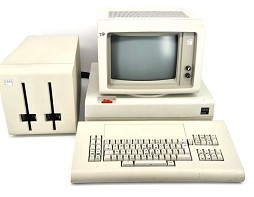
\includegraphics{./part-0/apparaetle.jpg}
\end{center}




%%%%%%%%%%%%%%%%%%%%%%%acknow.tex%%%%%%%%%%%%%%%%%%%%%%%%%%%%%%%%%%%%%%%%%
% sample acknowledgement chapter
%
% Use this file as a template for your own input.
%
%%%%%%%%%%%%%%%%%%%%%%%% Springer %%%%%%%%%%%%%%%%%%%%%%%%%%

\extrachap{Acknowledgements}

Use the template \emph{acknow.tex} together with the document class SVMono (monograph-type books) or SVMult (edited books) if you prefer to set your acknowledgement section as a separate chapter instead of including it as last part of your preface.



\tableofcontents

%

\chapter{Acronyms}

\begin{description}
\item[$E_{\mathbb{R}}$, $E_{\mathbb{C}} = E$] real, complex Banach lattice
\item[$E_{+}$] positive cone
\item[$E'$] dual
\item[$E^*$] semigroup dual
\item[$E_{F}^{T}$] F-product of E with respect to semigroup T
\item[$E_{F}$] F-product of E
\item[$E_{f}$] see C-I,4
\item[$(E,\phi)$] see C-I,4
\item[$E\otimes F$] tensor product
\item[$L(E)$] bounded linear operators on E
\item[$Z(E)$] center of E
\item[$E_{n}$] n-th Sobolev space
\item[$B(H)$] W*-algebra of bounded linear operators on H
\item[$S(M)$] state space of C*-algebra M
\item[$M_{+}$] positive cone of C*-algebra M
\item[$M_{*}$] predual
\item[$M^{sa}$] self-adjoint part
\item[$M_{n}$] C*-algebra of nxn-matrices
\item[AC] absolutely continuous functions
\item[BV] functions of bounded variation
\item[K] compact topological space
\item[X] locally compact topological space
\item[$C(K)$, $C(K,E)$] continuous functions (with values in E)
\item[$C_{o}(X)$, $C_{o}(X,E)$] continuous functions vanishing at infinity with values in E
\item[$C^{b}(X)$] bounded continuous functions
\item[$C_{uu}(X)$] uniformly continuous functions
\item[$C^{n}$, $C^{(n)}$] continuous differentiable functions (n-times)
\item[$C_{c}^{\infty}(\mathbb{R}^n)$] infinitely differentiable functions with compact support
\item[$L^{p}(\mu)$] p-integrable functions
\item[$S(\mathbb{R}^n)$] Schwartz space
\item[$M(K)$] regular Borel measures
\item[$M_{b}(X)$] bounded regular Borel measures
\item[$T = (T(t))_{t\geq0}$] (one-parameter) semigroup
\item[$T|$] subspace (reduced) semigroup
\item[$T/$] quotient semigroup
\item[Fix$(T)$] fixed space of T
\item[$A$] generator
\item[$A'$] adjoint
\item[$A^*$] adjoint generator
\item[$\sigma(A)$] spectrum
\item[$\rho(A)$] resolvent set
\item[$\sigma_{ess}(A)$] essential spectrum
\item[$\sigma_{b}(A)$] boundary spectrum
\item[$P\sigma(A)$] point spectrum
\item[$P\sigma_{b}(A)$] boundary point spectrum
\item[$A\sigma(A)$] approximate point spectrum
\item[$R\sigma(A)$] residual spectrum
\item[$\omega = \omega(A) = \omega(T)$] growth bound
\item[$s(A)$] spectral bound
\item[$\omega_{I}(A)$] growth bound of solution of (ACP)
\item[$\omega(f)$] growth bound of $T(\cdot)f$
\item[$r(T)$] spectral radius
\item[$\omega_{ess}(A)$] essential growth bound
\item[$r_{ess}(T)$] essential spectral radius
\item[$R(\lambda,A)$] resolvent operator
\item[$I^{d}$, $\{I^{d}\}_{d=1}^{dd}$] orthogonal band of I (of $I^{d}$)
\item[$\wedge$] infimum
\item[$\vee$] supremum
\item[$|T|$] modulus of regular operator
\item[$\hat{f}$, $\check{f}$] Fourier (inverse Fourier) transformation
\item[$d\rho(f)$] subdifferential of $\rho$ in f
\item[$dN(f)$] subdifferential of norm in f
\item[$dN^{+}(f)$] subdifferential of canonical half-norm in f
\item[im] range
\item[ker] null-space
\item[Im] imaginary part
\item[Re] real part
\item[$\text{Re}f$, $\text{Im}f$] see C-I,7
\item[$\text{Re}T$, $\text{Im}T$] see C-I,7
\item[$\bar{f}$] complex conjugate of f
\item[$S_{f}$] signum operator with respect to f
\item[sign $f$] signum of f
\item[$f^{[n]}$] see C-II,2.2
\item[$|f|$] absolute value of f
\item[$f^{+}$] positive part of f
\item[$f^{-}$] negative part of f
\item[Id] identity operator
\item[$M_{p}$] multiplication operator
\item[1] function identically 1
\item[$1_{C}$] characteristic function of set C
\item[$\delta_{x}$] Dirac measure in x
\item[tr] trace
\item[span M] linear subspace generated by M
\item[$S(\alpha)$] sector in complex plane
\item[(ACP)] abstract Cauchy problem
\item[(P)] positive minimum principle
\item[(P')] B-II,1.21
\item[(K)] Kato's (equality) inequality
\item[(RCP)] retarded Cauchy problem
\item[(RE)] retarded equation
\item[(T)] translation property
\end{description}


\mainmatter%%%%%%%%%%%%%%%%%%%%%%%%%%%%%%%%%%%%%%%%%%%%%%%%%%%%%%%

%% -- Part-A
% !TEX root = ../../LN-Book.tex
%% -- Stand 2025/01/13
%% -- ulgr
%% -- Part A
%% --

\begin{partbacktext}
\part[One-parameter Semigroups on Banach Spaces]{One-parameter Semigroups on \\Banach Spaces }
\end{partbacktext}
% !TEX root = LN-Book.tex
%% -- Stand 2025/01/13
%% -- ulgr
%% --
\chapter{Basic Results on Semigroups on Banach Spaces}
%% --
Since the basic theory of one-parameter semigroups can be found in several excellent books (e.g. Davies (1980), Goldstein (1985a), Pazy (1983) or Hille-Phillips (1957)) we do not want to give a self-contained introduction to this subject here.
It may however be useful to fix our notation, to collect briefly some important definitions and results (Section 1), to present a list of standard examples (Section 2) and to discuss standard constructions of new semigroups from a given one (Section 3).
In the entire chapter we denote by $E$ a (real or) complex Banach space and consider one-parameter semigroups of bounded linear operators $T(t)$ on $E$.
By this we understand a subset $\{T(t) \colon t \in \mathbb{R}_{+}\}$ of $L(E)$, usually written as $(T(t))_{t \geq 0}$, such that
%% --
\begin{align*}
	T(0) 	&= 	Id \\
	T(s+t) 	&= 	T(s) \cdot T(t) \text{ for all $s, t \in \mathbb{R}_{+}$.}
\end{align*}
%% --
In more abstract terms this means that the map $t \mapsto T(t)$ is a homomorphism from the additive semigroup $\mathbb{R}_{+}$ into the multiplicative semigroup $(L(E), \cdot)$.
Similarly, a one-parameter group $(T(t))_{t \in \mathbb{R}}$ will be a homomorphic image of the group $(\mathbb{R},+)$ in $(L(E), \cdot)$.
%% --
\section{Standard Definitions and Results}
%% --
We consider a one-parameter semigroup $(T(t))_{t \geq 0}$ on a Banach space $E$ and observe that the domain $\mathbb{R}_{+}$ and the range $L(E)$ of the (semigroup) homomorphism $\tau \colon t \mapsto T(t)$ are topological semigroups for the natural topology on $\mathbb{R}_{+}$ and any one of the standard operator topologies on $L(E)$.
We single out the strong operator topology on $L(E)$ and require $\tau$ to be continuous.
%% --
\begin{definition}
A one-parameter semigroup $(T(t))_{t \geq 0}$ is called strongly continuous if the map $t \mapsto T(t)$ is continuous for the strong operator topology on $L(E)$, i.e., $\lim_{t \to t_0} \|T(t)f - T(t_0)f\| = 0$ for every $f \in E$ and $t, t_0 \geq 0$.
\end{definition}
%% --
Clearly one defines in a similar way weakly continuous, resp. uniformly continuous (compare A-II, Def. 1.19) semigroups, but since we concentrate on the strongly continuous case we agree on the following terminology:
From now on \enquote*{semigroup} always means strongly continuous one-parameter semigroup of bounded linear operators.

Next we collect a few elementary facts on the continuity and boundedness of one-parameter semigroups.
%% --
\begin{remark}
%% --
\begin{enumerate}[(i)]
\item
A one-parameter semigroup $(T(t))_{t \geq 0}$ on a Banach space $E$ is strongly continuous if and only if for any $f \in E$ it is true that $T(t)f \to f$ as $t \to 0$.

\item
For every strongly continuous semigroup $(T(t))_{t \geq 0}$ there exist constants $M \geq 1$, $\omega \in \mathbb{R}$ such that $\|T(t)\| \leq M \cdot e^{\omega t}$ for every $t \geq 0$.

\item
If $(T(t))_{t \geq 0}$ is a one-parameter semigroup such that $\|T(t)\|$ is bounded for $0 \leq t \leq \delta$ then it is strongly continuous if and only if $\lim_{t \to 0} T(t)f = f$ for every $f$ in a total subset of $E$.

\end{enumerate}
%% --
\end{remark}
%% --
\begin{definition}
By the growth bound (or type) of the semigroup $(T(t))_{t \geq 0}$ we understand the number
%% --
\begin{align*}
\omega_{0} &:= \inf\{w \in \mathbb{R} \colon \text{There exists $ M \in \mathbb{R}_{+}$ such that $\|T(t)\| \leq M e^{wt}$ 
	for $t \geq 0$} \} \tag{*}\\
&= \lim_{t \to \infty} \frac{1}{t} \cdot \log\|T(t)\| = \inf_{t > 0} \frac{1}{t} \cdot \log\|T(t)\|
\end{align*}
\end{definition}
%% --
Particularly important are semigroups such that for every $t \geq 0$ we have $\|T(t)\| \leq M$ (bounded semigroups) or $\|T(t)\| \leq 1$ (contraction semigroups).
In both cases we have $\omega_{0} \leq 0$.

It follows from the subsequent examples and from 3.1 that $\omega_{0}$ may be any number $-\infty \leq \omega_{0} < +\infty$.
Moreover the reader should observe that the infimum in $ (*) $ need not be attained and that $M$ may be larger than $ 1 $ even for bounded semigroups.
%% --
\begin{example}
\begin{enumerate}[(i)]
\item
Take $E = \mathbb{C}^{2}$, $A = \begin{pmatrix} 0 & 1 \\ 0 & 0 \end{pmatrix}$ and $T(t) = e^{tA} = \begin{pmatrix} 1 & t \\ 0 & 1 \end{pmatrix}$.
Then for the $1$-norm on $E$ we obtain $\|T(t)\| = 1 + t$, hence $(T(t))_{t \geq 0}$ is an unbounded semigroup having growth bound $\omega_{0} = 0$.

\item
Take $E = L^{1}(\mathbb{R})$ and for $f \in E$ and $t \geq 0$ define
%% --
\[
	T(t)f(x) := \begin{cases}
		2 \cdot f(x+t) & \text{if } x \in [-t,0] \\
		f(x+t) & \text{otherwise.}
\end{cases}
\]
%% --
Each $T(t)$, $t > 0$, satisfies $\|T(t)\| = 2$ as can be seen by taking $f := 1_{[0,t]}$.
Therefore $(T(t))_{t \geq 0}$ is a strongly continuous semigroup which is bounded, hence has $\omega_{0} = 0$, but the constant $M$ in $ (*) $ cannot be chosen to be $ 1 $.

\end{enumerate}
\end{example}
%% --
\begin{definition}
To every semigroup $(T(t))_{t \geq 0}$ there belongs an operator $(A,D(A))$, called the generator and defined on the domain
\[
D(A) := \left\{f \in E \colon \lim_{h \to 0} \frac{T(h)f-f}{h} \text{ exists in } E\right\}
\]
by $Af := \lim_{h \to 0} \frac{T(h)f-f}{h}$ for $f \in D(A)$.
\end{definition}
%% --
Clearly, $D(A)$ is a linear subspace of $E$ and $A$ is linear from $D(A)$ into $E$.
Only in certain special cases (see 2.1) the generator is everywhere defined and therefore bounded (use Prop. 1.9(i)).
In general the precise extent of the domain $D(A)$ is essential for the characterisation of the generator.
But since the domain is canonically associated to the generator of a semigroup we shall write in most cases $A$ instead of $(A,D(A))$.
%% --
\begin{proposition}
For the generator $A$ of a semigroup $(T(t))_{t \geq 0}$ on a Banach space $E$ the following assertions hold:

\begin{enumerate}[(i)]
\item
If $f \in D(A)$ then $T(t)f \in D(A)$ for every $t \geq 0$.

\item
The map $t \mapsto T(t)f$ is differentiable on $\mathbb{R}_{+}$ if and only if $f \in D(A)$.
In that case one has
%% --
\begin{equation}
\frac{d}{dt}T(t)f = AT(t)f = T(t)Af.
\end{equation}
%% --
\item
Every $f \in E$ one has $\int_0^{t} T(s)f ds \in D(A)$ and
%% --
\begin{equation}
A\int_0^{t} T(s)f ds = T(t)f - f.
\end{equation}
%% --
\item
If $f \in D(A)$ then
%% --
\[
T(t)f = f + \int_0^{t} AT(s)f ds = f + \int_0^{t} T(s)Af ds.
\]
%% --
\item
The domain $D(A)$ is dense in $E$.

\end{enumerate}
\end{proposition}
%% --
\begin{theorem}
Let $(A,D(A))$ be the generator of a strongly continuous semigroup $(T(t))_{t \geq 0}$ on the Banach space $E$.
Then the \enquote*{abstract Cauchy problem} (ACP)
%% --
\[
\frac{d}{dt}\xi(t) = A\xi(t), \quad \xi(0) = f_0,
\]
has a unique solution $\xi \colon \mathbb{R}_{+} \to D(A)$ in $C^{1}(\mathbb{R}_{+},E)$ for every $f_0 \in D(A)$.
In fact, this solution is given by $\xi(t) := T(t)f_0$.
\end{theorem}
%% --
For the important relation of semigroups to abstract Cauchy problems we refer to A-II, Section 1.
Here we only point out that the above theorem implies that a semigroup is uniquely determined by its generator.
While the generator is bounded only for uniformly continuous semigroups (see 2.1 below), it always enjoys a weaker but useful property.
%% --
\begin{definition}
An operator $B$ with domain $D(B)$ on a Banach space $E$ is called closed if $D(B)$ endowed with the graph norm
\[
\|f\|_{B} := \|f\| + \|Bf\|
\]
becomes a Banach space.
Equivalently, $(B,D(B))$ is closed if and only if its graph $\{(f,Bf) \colon f \in D(B)\}$ is closed in $E \times E$, i.e.
\begin{equation}
f_{n} \in D(B), f_{n} \to f \text{ and } Bf_{n} \to g \text{ implies } f \in D(B) \text{ and } Bf = g.
\end{equation}
\end{definition}
%% --
It is clear from this definition that the \enquote*{closedness} of an operator $B$ depends very much on the size of the domain $D(B)$.
For example, a bounded and densely defined operator $(B,D(B))$ is closed if and only if $D(B) = E$.
On the other hand it may happen that $(B,D(B))$ is not closed but has a closed extension $(C,D(C))$, i.e., $D(B) \subset D(C)$ and $Bf = Cf$ for every $f \in D(B)$.
In that case, $B$ is called closable, a property which is equivalent to the following:
%% --
\begin{equation}
f_{n} \in D(B), f_{n} \to 0 \text{ and } Bf_{n} \to g \text{ implies } g = 0.
\end{equation}
%% --
The smallest closed extension of $(B,D(B))$ will be called the closure $\bar{B}$ with domain $D(\bar{B})$.
In other words, the graph of $\bar{B}$ is the closure of $\{(f,Bf) \colon f \in D(B)\}$ in $E \times E$.
Finally we call a subset $D_0$ of $D(B)$ a core for $B$ if $D_0$ is $\|\cdot\|_{B}$-dense in $D(B)$.
This means that a closed operator is determined (via closure) by its restriction to a core in its domain.
%% --
\begin{proposition}
For the generator $A$ of a strongly continuous semigroup $(T(t))_{t \geq 0}$ the following holds:

\begin{enumerate}[(i)]
\item
The generator $A$ is a closed operator.

\item
If a subspace $D_0$ of the domain $D(A)$ is dense in $E$ and $(T(t))$-invariant, then it is a core for $A$.
\item
Define $D(A^{n}) := \{f \in D(A^{n-1}) \colon Af \in D(A^{n-1})\}$, $D(A^{1}) = D(A)$.
Then $D(A^\infty) := \bigcap_{n \in \mathbb{N}} D(A^{n})$ is dense in $E$ and a core for $A$.

\end{enumerate}
\end{proposition}
%% --
\begin{example}
Property (iii) above does not hold for general densely defined closed operators.
Take $E = C[0,1]$, $D(B) = C^{1}[0,1]$ and $Bf = q \cdot f$ for some nowhere differentiable function $q \in C[0,1]$.
Then $B$ is closed, but $D(B^{2}) = (0)$.
\end{example}
%% --
\begin{proposition}
For the generator $A$ of a strongly continuous semigroup $(T(t))_{t \geq 0}$ on a Banach space $E$ the following holds.
If $\int_0^\infty e^{-\lambda t}T(t)f dt$ exists for every $f \in E$ and some $\lambda \in \mathbb{C}$, then $\lambda \in \rho(A)$ and $R(\lambda,A)f = \int_0^\infty e^{-\lambda t}T(t)f dt$.
In particular,
\begin{equation}
R(\lambda,A)^{n+1}f = \frac{(-1)^{n}}{n!}\left(\frac{d}{d\lambda}\right)^{n} R(\lambda,A)f = \int_0^\infty e^{-\lambda t}\frac{t^{n}}{n!}T(t)f dt
\end{equation}
for $n \in \mathbb{N}$, $f \in E$ and all $\lambda$ with $\operatorname{Re}\lambda > \omega$.
\end{proposition}
%% --
\begin{remark}

\begin{enumerate}[(i)]

\item
For continuous Banach space valued functions such as $t \mapsto T(t)f$ we consider the Riemann integral and define $\int_0^\infty T(t)f dt$ as $\lim_{t \to \infty} \int_0^{t} T(s)f ds$.
Sometimes such integrals for strongly continuous semigroups $(T(t))_{t \geq 0}$ are written as $\int_{a}^{b} T(t)dt$ and understood in the strong sense.

\item Since the generator $(A,D(A))$ determines the semigroup $(T(t))_{t > 0}$ uniquely, we will speak occasionally of the growth bound of the generator instead of the semigroup, i.e., we write $\omega = \omega(A) = \omega((T(t))_{t \geq 0})$.

\item
For one-parameter groups it might seem to be more natural to define the generator as the `derivative' rather than just the `right derivative' at $t = 0$.
This yields the same operator as the following result shows:
The strongly continuous semigroup $(T(t))_{t \geq 0}$ with generator $A$ can be extended to a strongly continuous one-parameter group $(U(t))_{t \in \mathbb{R}}$ if and only if $-A$ generates a semigroup $(S(t))_{t \geq 0}$.
In that case $(U(t))_{t \in \mathbb{R}}$ is obtained as
\[
U(t) := \begin{cases}
T(t) & \text{for } t \geq 0 \\
S(-t) & \text{for } t \leq 0
\end{cases}
\]
We refer to [Davies (1980), Prop.~1.14] for the details.

\end{enumerate}
\end{remark}

%% --
\section{Standard Examples}
In this section we list and discuss briefly the most basic examples of semigroups together with their generators.
These semigroups will reappear throughout this book and will be used to illustrate the theory.
We start with the class of semigroups mentioned after Definition 1.1.
%% --
\subsection{Uniformly Continuous Semigroups}
It follows from elementary operator theory that for every bounded operator $A \in L(E)$ the sum exists and determines a unique uniformly continuous (semi)group $(e^{tA})_{t \in \mathbb{R}}$ having $A$ as its generator.
%% --
\[
\sum_{n=0}^{m} \frac{t^n A^n}{n!} = \colon e^{tA}
\]
%% --
Conversely, any uniformly continuous semigroup is of this form: If the semigroup $(T(t))_{t \geq 0}$ is uniformly continuous, then $\frac{1}{t} \int_{0}^{t} T(s) ds$ uniformly converges to $T(0)=Id$ as $t \rightarrow 0$.
Therefore for some $t' \neq 0$ the operator $\frac{1}{t} \int_{0}^{t} T(s) ds$ is invertible and every $f \in E$ is of the form $f=\frac{1}{t} \int_{0}^{t'} T(s) g ds$ for some $g \in E$.
But these elements belong to $D(A)$ by (1.3), hence $D(A)=E$.
Since the generator $A$ is closed and everywhere defined it must be bounded.
Remark that bounded operators are always generators of groups, not just semigroups.
Moreover the growth bound $\omega$ satisfies $|\omega| \leq \|A\|$ in this situation.

The above characterization of the generators of uniformly continuous semigroups as the bounded operators shows that these semigroups are - at least in many aspects - rather simple objects.
%% --
\subsection{Matrix Semigroups}
The above considerations especially apply in the situation $E=\mathbb{C}^n$.
If $n=2$ and $A=(a_{ij})_{2\times 2}$ the following explicit formulas for $e^{tA}$ might be of interest:
Set $s:=\text{trace }A$, $d:=\text{det }A$ and $D:=(s^2-4d)^{1/2}$.
Then
%% --
\[
e^{tA}  = 
e^{ts/2} \cdot [D^{-1} 2\sinh(tD/2) \cdot A + (\cosh(tD/2)-sD^{-1}\sinh(tD/2)) \cdot Id]
\]
%% --
if $D \neq 0$ and
%% -- 
\[
e^{tA}  = 
e^{ts/2} \cdot [tA+(1-ts/2) \cdot Id] \text{\phantom{xxxxxxxxx}}
\]
%% --
if $D=\emptyset$ resp.
%% --
\subsection{Multiplication Semigroups}
Many Banach spaces appearing in applications are Banach spaces of (real or) complex valued functions over a set $X$.
As the most standard of these "function spaces", we mention the space $C_0(X)$ of all continuous complex valued functions vanishing at infinity on a locally compact space $X$, or the space $L^p(X,\Sigma,\mu), 1 \leq p \leq \infty$, of all (equivalence classes of) p-integrable functions on a $\sigma$-finite measure space $(X,\Sigma,\mu)$.

On these function spaces $E=C_0(X)$, resp. $E=L^p(X,\Sigma,\mu)$, there is a simple way to define \enquote{multiplication operators}: Take a continuous, resp. measurable function $q \colon X \rightarrow \mathbb{C}$ and define
%% --
\[
M_{q}f := q \cdot f, \text{ i.e. } M_{q}f(x) := q(x) \cdot f(x) \text{ for } x \in X,
\]
%% --
for every $f$ in the "maximal" domain $D(M_{q}) := \{g \in E \colon q \cdot g \in E\}$.

For such multiplication operators many properties can be checked quite directly.
For example, the following statements are equivalent:

\begin{enumerate}[(a)]
\item
$M_{q}$ is bounded.

\item
$q$ is (p-essentially) bounded.

\end{enumerate}
%% --
One has $\|M_{q}\| = \|q\|_\infty$ in this situation.

Observe that on spaces $C(K)$, $K$ compact, there are no densely defined, unbounded multiplication operators.

By defining the multiplication semigroups
%% --
\[
T(t)f(x) := \exp(t \cdot q(x))f(x), x \in X, f \in E,
\]
%% --
one obtains the following characterizations.

\begin{proposition} 
Let $M_{q}$ be a multiplication operator on $E=C_0(X)$ or $E=L^p(X,\Sigma,\mu), 1 \leq p < \infty$.
Then the properties (a) and (b), resp. $(a')$ and $(b')$, are equivalent:
\begin{enumerate}[(a)]
\item
$M_{q}$ generates a strongly continuous semigroup.
\item
$\sup\{\text{Re }q(x) \colon x \in X\} < \infty$.
\end{enumerate}
%% --

\begin{enumerate}[($a'$)]
\item
$M_{q}$ generates a uniformly continuous semigroup.
\item
$\sup\{|q(x)| \colon x \in X\} < \infty$.
\end{enumerate}
%% --
\end{proposition} 
As a consequence one computes the growth bound of a multiplication semigroup as follows:
\[
\omega = \sup\{\text{Re }q(x) \colon x \in X\} \text{ in the case } E = C_0(X),
\]
\[
\omega = \text{ess-sup}\{\text{Re }q(x) \colon x \in X\} \text{ in the case } E = L^p(\mu).
\]
%% --
It is a nice exercise to characterize those multiplication operators which generate strongly continuous groups.

\subsection{Translation (Semi)Groups}
Let $E$ be one of the following function spaces $C_0(\mathbb{R}_+)$, $C_0(\mathbb{R})$ or $L^p(\mathbb{R}_+)$, $L^p(\mathbb{R})$ for $1 \leq p < \infty$.
Define $T(t)$ to be the (left) translation operator
%% --
\[
T(t)f(x) := f(x+t)
\]
%% --
for $x,t \in \mathbb{R}_+$, resp. $x,t \in \mathbb{R}$ and $f \in E$.
Then $(T(t))_{t \geq 0}$ is a strongly continuous semigroup, resp. group of contractions on $E$ and its generator is the first derivative $\frac{d}{dx}$ with 'maximal' domain.
In order to be more precise we have to distinguish the cases $E=C_0$ and $E=L^p$:

\begin{enumerate}[(i)]

\item
The generator of the translation (semi)group on $E=C_0(\mathbb{R}_+)$ is
\[
Af := \frac{d}{dx}f = f',
\]
with domain 
\[
D(A) := \{f \in E \colon f \text{ differentiable and } f' \in E\}
\]
%% --
\begin{proof} For $f \in D(A)$ it follows that for every $x \in \mathbb{R}_{(+)}$
\[
\lim_{h \to 0} \frac{T(h)f(x)-f(x)}{h} = \lim_{h \to 0} \frac{f(x+h)-f(x)}{h} \text{ exists}
\]
%% --
(uniformly in $x$) and coincides with $Af(x)$.
Therefore $f$ is differentiable and $f' \in E$.
On the other hand, take $f \in E$ differentiable such that $f' \in E$.
Then
\[
\left|\frac{f(x+h)-f(x)}{h}-f'(x)\right| \leq \frac{1}{h} \int_{x}^{x+h}|f'(y)-f'(x)| dy
\]
%% --
where the last expression tends to zero uniformly in $x$ as $h \to 0$.
Thus $f \in D(A)$ and $f' = Af$.
\end{proof}

\item 
The generator of the translation (semi)group on $E=L^p(\mathbb{R}_{(+)}), 1 \leq p < \infty$, is
\[
Af := \frac{d}{dx}f = f',
\]
with domain
\[
D(A) := \{f \in E \colon f \text{ absolutely continuous}, f' \in E\}
\]
\end{enumerate}
%% --
\subsection{Rotation Groups}
On $E=C(\mathbb{T})$, resp. $E=L^p(\mathbb{T},m), 1 \leq p < \infty$, $m$ Lebesgue measure we have canonical groups defined by rotations of the unit circle $\mathbb{T}$ with a certain period.
For $0 < \tau \in \mathbb{R}$ the operators
%% --
\[
R_\tau(t)f(z) := f(e^{2\pi it/\tau} \cdot z)
\]
%% --
yield a group $(R_\tau(t))_{t \in \mathbb{R}}$ having period $\tau$, i.e. $R_\tau(\tau)=Id$.
As in Example 2.4 one shows that its generator has the form
%% --
\[
D(A) = \{f \in E \colon f \text{ absolutely continuous}, f' \in E\},
\]
\[
Af(z) = (2\pi i/\tau) \cdot z \cdot f'(z).
\]
%% --
An isomorphic copy of the group $(R_\tau(t))_{t \in \mathbb{R}}$ is obtained if we consider $E=\{f \in C[0,1] \colon f(0)=f(1)\}$, resp. $E=L^p([0,1])$ and the group of 'periodic translations'
%% --
\[
T(t)f(x) := f(y) \text{ for } y \in [0,1], y = x+t \text{ mod } 1
\]
%% --
with generator
%% --
\[
D(A) := \{f \in E \colon f \text{ absolutely continuous}, f' \in E\},
\]
\[
Af := f'.
\]
%% --
\subsection{Nilpotent Translation Semigroups}
Take $E=L^p([0,\tau],m)$ for $1 \leq p < \infty$ and define
%% --
\[
T(t)f(x) := \begin{cases}
f(x+t) & \text{if } x+t \leq \tau \\
0 & \text{otherwise}
\end{cases}
\]
%% --
Then $(T(t))_{t \geq 0}$ is a semigroup satisfying $T(t)=0$ for $t \geq \tau$.
Its generator is still the first derivative $A=\frac{d}{dx}$, but its domain is
\[
D(A) = \{f \in L^p([0,\tau]) \colon f \text{ absolutely continuous}, f' \in L^p([0,\tau]), f(\tau)=0\}.
\]
%% --
In fact, if $f \in D(A)$ then $f$ is absolutely continuous with $f' \in E$.
By Prop.1.6.i it follows that $T(t)f$ is absolutely continuous and hence $f(\tau)=0$.
%% --
\subsection{One-dimensional Diffusion Semigroup}
For the second derivative
%% --
\[
Bf(x) := \frac{d^2}{dx^2}f(x) = f''(x)
\]
%% --
we take the domain
\[
D(B) := \{f \in C^2[0,1] \colon f'(0)=f'(1)=0\}
\]
in the Banach space $E=C[0,1]$.
Then $D(B)$ is dense in $C[0,1]$, but closed for the graph norm.
Obviously, each function
%% --
\[
e_{n}(x) := \cos \pi nx, \quad n \in \mathbb{Z},
\]
%% --
is contained in $D(B)$ and an eigenfunction of $B$ pertaining to the eigenvalue $\lambda_{n} := -\pi^2n^2$.
The linear hull
\[
\text{span}\{e_{n} \colon n \in \mathbb{Z}\} = \colon E_0
\]
forms a subalgebra of $D(B)$ which by the Stone-Weierstrass theorem is dense in $E$.

We now use $e_{n}$ to define bounded linear operators
\[
e_{n} \otimes e_{n} \colon f \rightarrow \left(\int_0^1 f(x)e_{n}(x)dx\right)e_{n} = \langle f,e_{n}\rangle e_{n}
\]
satisfying $\|e_{n} \otimes e_{n}\| \leq 1$ and
$(e_{n} \otimes e_{n})(e_{m} \otimes e_{m}) = \delta_{n,m}(e_{n} \otimes e_{n})$ for $n \in \mathbb{Z}$.

For $t>0$ we define
\[
\begin{aligned}
T(t) &:= \sum_{n \in \mathbb{Z}} \exp(-\pi^2n^2t) \cdot e_{n} \otimes e_{n} \\
&= e_0 \otimes e_0 + 2\sum_{n=1}^{\infty} \exp(-\pi^2n^2t) \cdot e_{n} \otimes e_{n}
\end{aligned}
\]
%% --
or
%% --
\[
\begin{aligned}
T(t)f(x) &= \int_0^1 k_{t}(x,y)f(y)dy \\
&\text{where } k_{t}(x,y) = 1 + 2\sum_{n=1}^{\infty} \exp(-\pi^2n^2t)\cos \pi nx \cos \pi ny.
\end{aligned}
\]
%% --
Die Jacobi-Identität
\[
\begin{aligned}
w_{t}(x) &:= 1/(4\pi t)^{\frac{1}{2}} \sum_{m \in \mathbb{Z}} \exp(-(x+2m)^2/4t) \\
&= \frac{1}{2} + \sum_{n \in \mathbb{N}} \exp(-\pi^2n^2t)\cos \pi nx
\end{aligned}
\]
%% --
und trigonometrische Beziehungen zeigen, dass
\[
k_{t}(x,y) = w_{t}(x+y) + w_{t}(x-y)
\]
%% --
welches eine positive Funktion auf $[0,1]^2$ ist.
Daher ist $T(t)$ ein beschränkter Operator auf $C[0,1]$ mit
\[
\|T(t)\| = \|T(t)1\| = \sup_{x \in [0,1]} \int_0^1 k_{t}(x,y)dy = 1.
\]
%% --
\subsection{n-dimensional Diffusion Semigroup}
On $E=L^p(\mathbb{R}^n), 1 \leq p < \infty$, the operators
%% --
\[
\begin{aligned}
T(t)f(x) &:= (4\pi t)^{-n/2} \int_{\mathbb{R}^n} \exp(-|x-y|^2/4t)f(y)dy \\
&:= \psi_{t} * f(x)
\end{aligned}
\]
%% --
for $x \in \mathbb{R}^n$, $t>0$ and $\psi_{t}(x) := (4\pi t)^{-n/2}\exp(-|x|^2/4t)$ form a strongly continuous semigroup.

In fact the integral exists for every $f \in L^p(\mathbb{R}^n)$, since $\psi_{t}$ is an element of the Schwartz space $\mathcal{S}(\mathbb{R}^n)$ of all rapidly decreasing smooth functions on $\mathbb{R}^n$.

Moreover,
\[
\|T(t)f\|_{p} \leq \|\psi_{t}\|_{1}\|f\|_{p} = \|f\|_{p}
\]
%% --
by Young's inequality [Reed-Simon (1975), p.28], hence $\|T(t)\| \leq 1$ for every $t>0$.

Next we observe that $\mathcal{S}(\mathbb{R}^n)$ is dense in $E$ and invariant under each $T(t)$.
Therefore we can apply the Fourier transformation $\mathcal{F}$ which leaves $\mathcal{S}(\mathbb{R}^n)$ invariant and yields
\[
\mathcal{F}(\psi_{t} * f) = (2\pi)^{n/2}\mathcal{F}(\psi_{t}) \cdot \mathcal{F}(f) = (2\pi)^{n/2}\hat{\psi_{t}} \cdot \hat{f}
\]
where $f \in \mathcal{S}(\mathbb{R}^n)$, $\hat{f} = \mathcal{F}f \in \mathcal{S}(\mathbb{R}^n)$.

In other words, $\mathcal{F}$ transforms $(T(t)|_{\mathcal{S}(\mathbb{R}^n)})_{t \geq 0}$ into a multiplication semigroup on $\mathcal{S}(\mathbb{R}^n)$ which is pointwise continuous for the usual topology of $\mathcal{S}(\mathbb{R}^n)$.
The generator, i.e. the right derivative at 0, of this semigroup is the multiplication operator
\[
B\hat{f}(x) := -|x|^2\hat{f}(x)
\]
for every $f \in \mathcal{S}(\mathbb{R}^n)$.

Applying the inverse Fourier transformation and observing that the topology of $\mathcal{S}(\mathbb{R}^n)$ is finer than the topology induced from $L^p(\mathbb{R}^n)$, we obtain that $(T(t))_{t \geq 0}$ is a semigroup which is strongly continuous (use Remark 1.2, (3)) and its generator $A$ coincides with
\[
\Delta f(x) = \sum_{i=1}^n \frac{\partial^2}{\partial x_{i}^2}f(x_{1},\ldots,x_{n})
\]
for every $f \in \mathcal{S}(\mathbb{R}^n)$.

Since $\mathcal{S}(\mathbb{R}^n)$ is $(T(t))$-invariant we have determined the generator on a core of its domain (see Prop.1.9.ii).

In particular the above semigroup 'solves' the initial value problem for the 'heat equation'
\[
\frac{\partial}{\partial t}f(x,t) = \Delta f(x,t), \quad f(x,0) = f_0(x), \quad x \in \mathbb{R}^n.
\]
%% --
For the analogous discussion of the unitary group on $L^2(\mathbb{R}^n)$ generated by
\[
C := i\Delta
\]
we refer to Section IX.7 in Reed-Simon (1975).

%% --

\section{Standard Constructions}
Starting with a semigroup $(T(t))_{t \geq 0}$ on a Banach space $E$ it is possible to construct new semigroups on spaces naturally associated with $E$.
Such constructions will be important technical devices in many of the subsequent proofs.
Although most of these constructions are rather routine, we present in the sequel a systematic account of them for the convenience of the reader.

We always start with a semigroup $(T(t))_{t \geq 0}$ on a Banach space $E$, and denote its generator by $A$ on the domain $D(A)$.

\subsection{Similar Semigroups}
There is an easy way how to obtain different (but isomorphic) semigroups: Take any isomorphism $S \in L(E,F)$ between two Banach spaces $E$ and $F$.
Then
\[
U(t) := ST(t)S^{-1}, \quad t \geq 0,
\]
defines a semigroup on $F$ which is strongly continuous if and only if $(T(t))_{t \geq 0}$ has this property.
In this case the generator $B$ of $(U(t))_{t \geq 0}$ is given by
\[
B = SAS^{-1} \text{ with } D(B) = SD(A).
\]

%%%%%%%%%%%%%%%%%%%%%% appendix.tex %%%%%%%%%%%%%%%%%%%%%%%%%%%%%%%%%
%
% sample appendix
%
% Use this file as a template for your own input.
%
%%%%%%%%%%%%%%%%%%%%%%%% Springer-Verlag %%%%%%%%%%%%%%%%%%%%%%%%%%

\chapter{Chapter Heading}
\label{introA} % Always give a unique label
% use \chaptermark{}
% to alter or adjust the chapter heading in the running head

Use the template \emph{appendix.tex} together with the document class SVMono (monograph-type books) or SVMult (edited books) to style appendix of your book.


\section{Section Heading}
\label{sec:A1}
% Always give a unique label
% and use \ref{<label>} for cross-references
% and \cite{<label>} for bibliographic references
% use \sectionmark{}
% to alter or adjust the section heading in the running head
Instead of simply listing headings of different levels we recommend to let every heading be followed by at least a short passage of text. Further on please use the \LaTeX\ automatism for all your cross-references and citations.


\subsection{Subsection Heading}
\label{sec:A2}
Instead of simply listing headings of different levels we recommend to let every heading be followed by at least a short passage of text. Further on please use the \LaTeX\ automatism for all your cross-references and citations as has already been described in Sect.~\ref{sec:A1}.

For multiline equations we recommend to use the \verb|eqnarray| environment.
\begin{eqnarray}
\vec{a}\times\vec{b}=\vec{c} \nonumber\\
\vec{a}\times\vec{b}=\vec{c}
\label{eq:A01}
\end{eqnarray}

\subsubsection{Subsubsection Heading}
Instead of simply listing headings of different levels we recommend to let every heading be followed by at least a short passage of text. Further on please use the \LaTeX\ automatism for all your cross-references and citations as has already been described in Sect.~\ref{sec:A2}.

Please note that the first line of text that follows a heading is not indented, whereas the first lines of all subsequent paragraphs are.

% For figures use
%
\begin{figure}[t]
\sidecaption[t]
% Use the relevant command for your figure-insertion program
% to insert the figure file.
% For example, with the graphicx style use
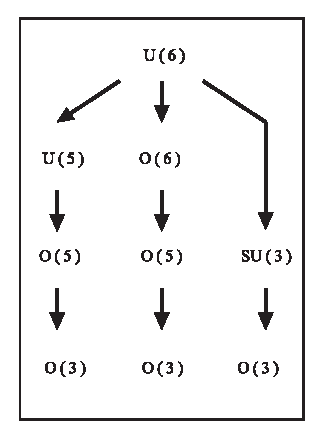
\includegraphics[scale=.65]{figure}
%
% If no graphics program available, insert a blank space i.e. use
%\picplace{5cm}{2cm} % Give the correct figure height and width in cm
%
\caption{Please write your figure caption here}
\label{fig:A1}       % Give a unique label
\end{figure}

% For tables use
%
\begin{table}
\caption{Please write your table caption here}
\label{tab:A1}       % Give a unique label
%
% Follow this input for your own table layout
%
\begin{tabular}{p{2cm}p{2.4cm}p{2cm}p{4.9cm}}
\hline\noalign{\smallskip}
Classes & Subclass & Length & Action Mechanism  \\
\noalign{\smallskip}\hline\noalign{\smallskip}
Translation & mRNA$^a$  & 22 (19--25) & Translation repression, mRNA cleavage\\
Translation & mRNA cleavage & 21 & mRNA cleavage\\
Translation & mRNA  & 21--22 & mRNA cleavage\\
Translation & mRNA  & 24--26 & Histone and DNA Modification\\
\noalign{\smallskip}\hline\noalign{\smallskip}
\end{tabular}
$^a$ Table foot note (with superscript)
\end{table}
%


%% -- Part-B
% !TEX root = ../../LN-Book.tex
%% -- Stand 2025/01/13
%% -- ulgr
%% -- Part B
%% --
\begin{partbacktext}
\part{Positive Semigroups on Spaces $C_{0}(X)$}
\end{partbacktext}
\setcounter{chapter}{0}
%%%%%%%%%%%%%%%%%%%%%% chapter.tex %%%%%%%%%%%%%%%%%%%%%%%%%%%%%%%%%
%
% sample chapter
%
% Use this file as a template for your own input.
%
%%%%%%%%%%%%%%%%%%%%%%%% Springer-Verlag %%%%%%%%%%%%%%%%%%%%%%%%%%
%\motto{Use the template \emph{chapter.tex} to style the various elements of your chapter content.}
\chapter{Chapter Heading}
\label{intro} % Always give a unique label
% use \chaptermark{}
% to alter or adjust the chapter heading in the running head

\abstract*{Each chapter should be preceded by an abstract (no more than 200 words) that summarizes the content. The abstract will appear \textit{online} at \url{www.SpringerLink.com} and be available with unrestricted access. This allows unregistered users to read the abstract as a teaser for the complete chapter.
Please use the 'starred' version of the new \texttt{abstract} command for typesetting the text of the online abstracts (cf. source file of this chapter template \texttt{abstract}) and include them with the source files of your manuscript. Use the plain \texttt{abstract} command if the abstract is also to appear in the printed version of the book.}

\abstract{Each chapter should be preceded by an abstract (no more than 200 words) that summarizes the content. The abstract will appear \textit{online} at \url{www.SpringerLink.com} and be available with unrestricted access. This allows unregistered users to read the abstract as a teaser for the complete chapter. \newline\indent
Please use the 'starred' version of the new \texttt{abstract} command for typesetting the text of the online abstracts (cf. source file of this chapter template \texttt{abstract}) and include them with the source files of your manuscript. Use the plain \texttt{abstract} command if the abstract is also to appear in the printed version of the book.}

\section{Section Heading}
\label{sec:1}
Use the template \emph{chapter.tex} together with the document class SVMono (monograph-type books) or SVMult (edited books) to style the various elements of your chapter content conformable to the Springer Nature layout.

\section{Section Heading}
\label{sec:2}
% Always give a unique label
% and use \ref{<label>} for cross-references
% and \cite{<label>} for bibliographic references
% use \sectionmark{}
% to alter or adjust the section heading in the running head
Instead of simply listing headings of different levels we recommend to let every heading be followed by at least a short passage of text. Furtheron please use the \LaTeX\ automatism for all your cross-references and citations.

Please note that the first line of text that follows a heading is not indented, whereas the first lines of all subsequent paragraphs are.

\eject

Use the standard \verb|equation| environment to typeset your equations, e.g.
%
\begin{equation}
a \times b = c\;,
\end{equation}
%
however, for multiline equations we recommend to use the \verb|eqnarray| environment\footnote{In physics texts please activate the class option \texttt{vecphys} to depict your vectors in \textbf{\itshape boldface-italic} type - as is customary for a wide range of physical subjects.}.
\begin{eqnarray}
\left|\nabla U_{\alpha}^{\mu}(y)\right| &\le&\frac1{d-\alpha}\int
\left|\nabla\frac1{|\xi-y|^{d-\alpha}}\right|\,d\mu(\xi) =
\int \frac1{|\xi-y|^{d-\alpha+1}} \,d\mu(\xi)\qquad  \\
&=&(d-\alpha+1) \int\limits_{d(y)}^\infty
\frac{\mu(B(y,r))}{r^{d-\alpha+2}}\,dr \le (d-\alpha+1)
\int\limits_{d(y)}^\infty \frac{r^{d-\alpha}}{r^{d-\alpha+2}}\,dr
\label{eq:01}
\end{eqnarray}

\enlargethispage{24pt}

\subsection{Subsection Heading}
\label{subsec:2}
Instead of simply listing headings of different levels we recommend to let every heading be followed by at least a short passage of text. Further on please use the \LaTeX\ automatism for all your cross-references\index{cross-references} and citations\index{citations} as has already been described in Sect.~\ref{sec:2}.

\begin{quotation}
Please do not use quotation marks when quoting texts! Simply use the \verb|quotation| environment -- it will automatically be rendered in the preferred layout.
\end{quotation}


\subsubsection{Subsubsection Heading}
Instead of simply listing headings of different levels we recommend to let every heading be followed by at least a short passage of text. Furtheron please use the \LaTeX\ automatism for all your cross-references and citations as has already been described in Sect.~\ref{subsec:2}, see also Fig.~\ref{fig:1}\footnote{If you copy text passages, figures, or tables from other works, you must obtain \textit{permission} from the copyright holder (usually the original publisher). Please enclose the signed permission with the manucript. The sources\index{permission to print} must be acknowledged either in the captions, as footnotes or in a separate section of the book.}

Please note that the first line of text that follows a heading is not indented, whereas the first lines of all subsequent paragraphs are.

% For figures use
%
\begin{figure}[b]
\sidecaption
% Use the relevant command for your figure-insertion program
% to insert the figure file.
% For example, with the option graphics use
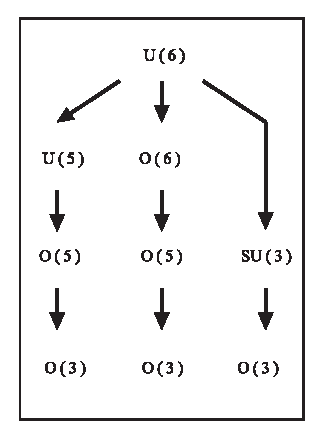
\includegraphics[scale=.65]{figure}
%
% If not, use
%\picplace{5cm}{2cm} % Give the correct figure height and width in cm
%
\caption{If the width of the figure is less than 7.8 cm use the \texttt{sidecapion} command to flush the caption on the left side of the page. If the figure is positioned at the top of the page, align the sidecaption with the top of the figure -- to achieve this you simply need to use the optional argument \texttt{[t]} with the \texttt{sidecaption} command}
\label{fig:1}       % Give a unique label
\end{figure}


\paragraph{Paragraph Heading} %
Instead of simply listing headings of different levels we recommend to let every heading be followed by at least a short passage of text. Furtheron please use the \LaTeX\ automatism for all your cross-references and citations as has already been described in Sect.~\ref{sec:2}.

Please note that the first line of text that follows a heading is not indented, whereas the first lines of all subsequent paragraphs are.

For typesetting numbered lists we recommend to use the \verb|enumerate| environment -- it will automatically render Springer's preferred layout.

\begin{enumerate}
\item{Livelihood and survival mobility are oftentimes coutcomes of uneven socioeconomic development.}
\begin{enumerate}
\item{Livelihood and survival mobility are oftentimes coutcomes of uneven socioeconomic development.}
\item{Livelihood and survival mobility are oftentimes coutcomes of uneven socioeconomic development.}
\end{enumerate}
\item{Livelihood and survival mobility are oftentimes coutcomes of uneven socioeconomic development.}
\end{enumerate}


\subparagraph{Subparagraph Heading} In order to avoid simply listing headings of different levels we recommend to let every heading be followed by at least a short passage of text. Use the \LaTeX\ automatism for all your cross-references and citations as has already been described in Sect.~\ref{sec:2}, see also Fig.~\ref{fig:2}.

Please note that the first line of text that follows a heading is not indented, whereas the first lines of all subsequent paragraphs are.

For unnumbered list we recommend to use the \verb|itemize| environment -- it will automatically render Springer's preferred layout.

\begin{itemize}
\item{Livelihood and survival mobility are oftentimes coutcomes of uneven socioeconomic development, cf. Table~\ref{tab:1}.}
\begin{itemize}
\item{Livelihood and survival mobility are oftentimes coutcomes of uneven socioeconomic development.}
\item{Livelihood and survival mobility are oftentimes coutcomes of uneven socioeconomic development.}
\end{itemize}
\item{Livelihood and survival mobility are oftentimes coutcomes of uneven socioeconomic development.}
\end{itemize}

\begin{figure}[t]
\sidecaption[t]
% Use the relevant command for your figure-insertion program
% to insert the figure file.
% For example, with the option graphics use
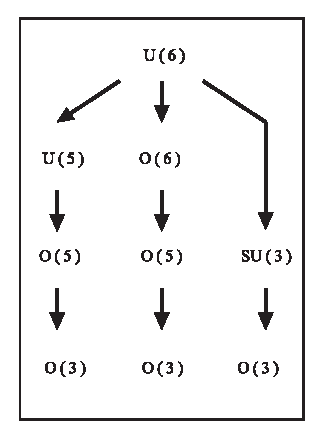
\includegraphics[scale=.65]{figure}
%
% If not, use
%\picplace{5cm}{2cm} % Give the correct figure height and width in cm
%
\caption{Please write your figure caption here}
\label{fig:2}       % Give a unique label
\end{figure}

\runinhead{Run-in Heading Boldface Version} Use the \LaTeX\ automatism for all your cross-references and citations as has already been described in Sect.~\ref{sec:2}.

\subruninhead{Run-in Heading Boldface and Italic Version} Use the \LaTeX\ automatism for all your cross-refer\-ences and citations as has already been described in Sect.~\ref{sec:2}\index{paragraph}.

\subsubruninhead{Run-in Heading Displayed Version} Use the \LaTeX\ automatism for all your cross-refer\-ences and citations as has already been described in Sect.~\ref{sec:2}\index{paragraph}.
% Use the \index{} command to code your index words
%
% For tables use
%
\begin{table}[!t]
\caption{Please write your table caption here}
\label{tab:1}       % Give a unique label
%
% For LaTeX tables use
%
\begin{tabular}{p{2cm}p{2.4cm}p{2cm}p{4.9cm}}
\hline\noalign{\smallskip}
Classes & Subclass & Length & Action Mechanism  \\
\noalign{\smallskip}\svhline\noalign{\smallskip}
Translation & mRNA$^a$  & 22 (19--25) & Translation repression, mRNA cleavage\\
Translation & mRNA cleavage & 21 & mRNA cleavage\\
Translation & mRNA  & 21--22 & mRNA cleavage\\
Translation & mRNA  & 24--26 & Histone and DNA Modification\\
\noalign{\smallskip}\hline\noalign{\smallskip}
\end{tabular}
$^a$ Table foot note (with superscript)
\end{table}
%
\section{Section Heading}
\label{sec:3}
% Always give a unique label
% and use \ref{<label>} for cross-references
% and \cite{<label>} for bibliographic references
% use \sectionmark{}
% to alter or adjust the section heading in the running head
Instead of simply listing headings of different levels we recommend to let every heading be followed by at least a short passage of text. Furtheron please use the \LaTeX\ automatism for all your cross-references and citations as has already been described in Sect.~\ref{sec:2}.

Please note that the first line of text that follows a heading is not indented, whereas the first lines of all subsequent paragraphs are.

If you want to list definitions or the like we recommend to use the Springer-enhanced \verb|description| environment -- it will automatically render Springer's preferred layout.

\begin{description}[Type 1]
\item[Type 1]{That addresses central themes pertainng to migration, health, and disease. In Sect.~\ref{sec:1}, Wilson discusses the role of human migration in infectious disease distributions and patterns.}
\item[Type 2]{That addresses central themes pertainng to migration, health, and disease. In Sect.~\ref{subsec:2}, Wilson discusses the role of human migration in infectious disease distributions and patterns.}
\end{description}

\subsection{Subsection Heading} %
In order to avoid simply listing headings of different levels we recommend to let every heading be followed by at least a short passage of text. Use the \LaTeX\ automatism for all your cross-references and citations citations as has already been described in Sect.~\ref{sec:2}.

Please note that the first line of text that follows a heading is not indented, whereas the first lines of all subsequent paragraphs are.

\begin{svgraybox}
If you want to emphasize complete paragraphs of texts we recommend to use the newly defined Springer class option \verb|graybox| and the newly defined environment \verb|svgraybox|. This will produce a 15 percent screened box 'behind' your text.

If you want to emphasize complete paragraphs of texts we recommend to use the newly defined Springer class option and environment \verb|svgraybox|. This will produce a 15 percent screened box 'behind' your text.
\end{svgraybox}


\subsubsection{Subsubsection Heading}
Instead of simply listing headings of different levels we recommend to let every heading be followed by at least a short passage of text. Furtheron please use the \LaTeX\ automatism for all your cross-references and citations as has already been described in Sect.~\ref{sec:2}.

Please note that the first line of text that follows a heading is not indented, whereas the first lines of all subsequent paragraphs are.

\begin{theorem}
Theorem text goes here.
\end{theorem}
%
% or
%
\begin{definition}
Definition text goes here.
\end{definition}

\begin{proof}
%\smartqed
Proof text goes here.
%\qed
\end{proof}

\paragraph{Paragraph Heading} %
Instead of simply listing headings of different levels we recommend to let every heading be followed by at least a short passage of text. Furtheron please use the \LaTeX\ automatism for all your cross-references and citations as has already been described in Sect.~\ref{sec:2}.

Note that the first line of text that follows a heading is not indented, whereas the first lines of all subsequent paragraphs are.
%
% For built-in environments use
%
\begin{theorem}
Theorem text goes here.
\end{theorem}
%
\begin{definition}
Definition text goes here.
\end{definition}
%
\begin{proof}
%\smartqed
Proof text goes here.
%\qed
\end{proof}
%
%
\begin{trailer}{Trailer Head}
If you want to emphasize complete paragraphs of texts in a \verb|Trailer Head| we recommend to
use  \begin{verbatim}\begin{trailer}{Trailer Head}
...
\end{trailer}\end{verbatim}
\end{trailer}
%
\begin{questype}{Questions}
If you want to emphasize complete paragraphs of texts in an \verb|Questions| we recommend to
use  \begin{verbatim}\begin{questype}{Questions}
...
\end{questype}\end{verbatim}
\end{questype}
%
%
\begin{important}{Important}
If you want to emphasize complete paragraphs of texts in an \verb|Important| we recommend to
use  \begin{verbatim}\begin{important}{Important}
...
\end{important}\end{verbatim}
\end{important}
%
\clearpage
\begin{warning}{Attention}
If you want to emphasize complete paragraphs of texts in an \verb|Attention| we recommend to
use  \begin{verbatim}\begin{warning}{Attention}
...
\end{warning}\end{verbatim}
\end{warning}

\begin{programcode}{Program Code}
If you want to emphasize complete paragraphs of texts in a \verb|Program Code| we recommend to
use

\verb|\begin{programcode}{Program Code}|

\verb|\begin{verbatim}...\end{verbatim}|

\verb|\end{programcode}|

\end{programcode}
%
\begin{tips}{Tips}
If you want to emphasize complete paragraphs of texts in a \verb|Tips| we recommend to
use  \begin{verbatim}\begin{tips}{Tips}
...
\end{tips}\end{verbatim}
\end{tips}
%
%
\begin{overview}{Overview}
If you want to emphasize complete paragraphs of texts in an \verb|Overview| we recommend to
use  \begin{verbatim}\begin{overview}{Overview}
...
\end{overview}\end{verbatim}
\end{overview}
\clearpage
\begin{backgroundinformation}{Background Information}
If you want to emphasize complete paragraphs of texts in a \verb|Background|
\verb|Information| we recommend to
use

\verb|\begin{backgroundinformation}{Background Information}|

\verb|...|

\verb|\end{backgroundinformation}|
\end{backgroundinformation}
\begin{legaltext}{Legal Text}
If you want to emphasize complete paragraphs of texts in a \verb|Legal Text| we recommend to
use  \begin{verbatim}\begin{legaltext}{Legal Text}
...
\end{legaltext}\end{verbatim}
\end{legaltext}
%
\begin{acknowledgement}
If you want to include acknowledgments of assistance and the like at the end of an individual chapter please use the \verb|acknowledgement| environment -- it will automatically render Springer's preferred layout.
\end{acknowledgement}
%
\section*{Appendix}
\addcontentsline{toc}{section}{Appendix}
%
When placed at the end of a chapter or contribution (as opposed to at the end of the book), the numbering of tables, figures, and equations in the appendix section continues on from that in the main text. Hence please \textit{do not} use the \verb|appendix| command when writing an appendix at the end of your chapter or contribution. If there is only one the appendix is designated ``Appendix'', or ``Appendix 1'', or ``Appendix 2'', etc. if there is more than one.

\begin{equation}
a \times b = c
\end{equation}
% Problems or Exercises should be sorted chapterwise
\section*{Problems}
\addcontentsline{toc}{section}{Problems}
%
% Use the following environment.
% Don't forget to label each problem;
% the label is needed for the solutions' environment
\begin{prob}
\label{prob1}
A given problem or Excercise is described here. The
problem is described here. The problem is described here.
\end{prob}

\begin{prob}
\label{prob2}
\textbf{Problem Heading}\\
(a) The first part of the problem is described here.\\
(b) The second part of the problem is described here.
\end{prob}

%%%%%%%%%%%%%%%%%%%%%%%% referenc.tex %%%%%%%%%%%%%%%%%%%%%%%%%%%%%%
% sample references
% %
% Use this file as a template for your own input.
%
%%%%%%%%%%%%%%%%%%%%%%%% Springer-Verlag %%%%%%%%%%%%%%%%%%%%%%%%%%
%
% BibTeX users please use
% \bibliographystyle{}
% \bibliography{}
%
%\biblstarthook{
\section{Styling of References}
In view of the parallel print and (chapter-wise) online publication of your book at \url{www.springerlink.com} it has been decided that -- as a genreral rule --  references should be sorted chapter-wise and placed at the end of the individual chapters. However, upon agreement with your contact at Springer you may list your references in a single seperate chapter at the end of your book. Deactivate the class option \texttt{sectrefs} and the \texttt{thebibliography} environment will be put out as a chapter of its own.\\\indent
References may be \textit{cited} in the text either by number (preferred) or by author/year.\footnote{Make sure that all references from the list are cited in the text. Those not cited should be moved to a separate \textit{Further Reading} section or chapter.} If the citatiion in the text is numbered, the reference list should be arranged in ascending order. If the citation in the text is author/year, the reference list should be \textit{sorted} alphabetically and if there are several works by the same author, the following order should be used:
\begin{enumerate}
\item all works by the author alone, ordered chronologically by year of publication
\item all works by the author with a coauthor, ordered alphabetically by coauthor
\item all works by the author with several coauthors, ordered chronologically by year of publication.
\end{enumerate}
The \textit{styling} of references\footnote{Always use the standard abbreviation of a journal's name according to the ISSN \textit{List of Title Word Abbreviations}, see \url{http://www.issn.org/en/node/344}} depends on the subject of your book:
\begin{itemize}
\item The \textit{two} recommended styles for references in books on \textit{mathematical, physical, statistical and computer sciences} are depicted in ~\cite{science-contrib, science-online, science-mono, science-journal, science-DOI} and ~\cite{phys-online, phys-mono, phys-journal, phys-DOI, phys-contrib}.
\item Examples of the most commonly used reference style in books on \textit{Psychology, Social Sciences} are~\cite{psysoc-mono, psysoc-online,psysoc-journal, psysoc-contrib, psysoc-DOI}.
\item Examples for references in books on \textit{Humanities, Linguistics, Philosophy} are~\cite{humlinphil-journal, humlinphil-contrib, humlinphil-mono, humlinphil-online, humlinphil-DOI}.
\item Examples of the basic Springer style used in publications on a wide range of subjects such as \textit{Computer Science, Economics, Engineering, Geosciences, Life Sciences, Medicine, Biomedicine} are ~\cite{basic-contrib, basic-online, basic-journal, basic-DOI, basic-mono}. 
\end{itemize}
%}

\begin{thebibliography}{99.}%
% and use \bibitem to create references.
%
% Use the following syntax and markup for your references if 
% the subject of your book is from the field 
% "Mathematics, Physics, Statistics, Computer Science"
%
% Contribution 
\bibitem{science-contrib} Broy, M.: Software engineering --- from auxiliary to key technologies. In: Broy, M., Dener, E. (eds.) Software Pioneers, pp. 10-13. Springer, Heidelberg (2002)
%
% Online Document
\bibitem{science-online} Dod, J.: Effective substances. In: The Dictionary of Substances and Their Effects. Royal Society of Chemistry (1999) Available via DIALOG. \\
\url{http://www.rsc.org/dose/title of subordinate document. Cited 15 Jan 1999}
%
% Monograph
\bibitem{science-mono} Geddes, K.O., Czapor, S.R., Labahn, G.: Algorithms for Computer Algebra. Kluwer, Boston (1992) 
%
% Journal article
\bibitem{science-journal} Hamburger, C.: Quasimonotonicity, regularity and duality for nonlinear systems of partial differential equations. Ann. Mat. Pura. Appl. \textbf{169}, 321--354 (1995)
%
% Journal article by DOI
\bibitem{science-DOI} Slifka, M.K., Whitton, J.L.: Clinical implications of dysregulated cytokine production. J. Mol. Med. (2000) doi: 10.1007/s001090000086 
%
%\bigskip

% Use the following (APS) syntax and markup for your references if 
% the subject of your book is from the field 
% "Mathematics, Physics, Statistics, Computer Science"
%
% Online Document
\bibitem{phys-online} J. Dod, in \textit{The Dictionary of Substances and Their Effects}, Royal Society of Chemistry. (Available via DIALOG, 1999), 
\url{http://www.rsc.org/dose/title of subordinate document. Cited 15 Jan 1999}
%
% Monograph
\bibitem{phys-mono} H. Ibach, H. L\"uth, \textit{Solid-State Physics}, 2nd edn. (Springer, New York, 1996), pp. 45-56 
%
% Journal article
\bibitem{phys-journal} S. Preuss, A. Demchuk Jr., M. Stuke, Appl. Phys. A \textbf{61}
%
% Journal article by DOI
\bibitem{phys-DOI} M.K. Slifka, J.L. Whitton, J. Mol. Med., doi: 10.1007/s001090000086
%
% Contribution 
\bibitem{phys-contrib} S.E. Smith, in \textit{Neuromuscular Junction}, ed. by E. Zaimis. Handbook of Experimental Pharmacology, vol 42 (Springer, Heidelberg, 1976), p. 593
%
%\bigskip
%
% Use the following syntax and markup for your references if 
% the subject of your book is from the field 
% "Psychology, Social Sciences"
%
%
% Monograph
\bibitem{psysoc-mono} Calfee, R.~C., \& Valencia, R.~R. (1991). \textit{APA guide to preparing manuscripts for journal publication.} Washington, DC: American Psychological Association.
%
% Online Document
\bibitem{psysoc-online} Dod, J. (1999). Effective substances. In: The dictionary of substances and their effects. Royal Society of Chemistry. Available via DIALOG. \\
\url{http://www.rsc.org/dose/Effective substances.} Cited 15 Jan 1999.
%
% Journal article
\bibitem{psysoc-journal} Harris, M., Karper, E., Stacks, G., Hoffman, D., DeNiro, R., Cruz, P., et al. (2001). Writing labs and the Hollywood connection. \textit{J Film} Writing, 44(3), 213--245.
%
% Contribution 
\bibitem{psysoc-contrib} O'Neil, J.~M., \& Egan, J. (1992). Men's and women's gender role journeys: Metaphor for healing, transition, and transformation. In B.~R. Wainrig (Ed.), \textit{Gender issues across the life cycle} (pp. 107--123). New York: Springer.
%
% Journal article by DOI
\bibitem{psysoc-DOI}Kreger, M., Brindis, C.D., Manuel, D.M., Sassoubre, L. (2007). Lessons learned in systems change initiatives: benchmarks and indicators. \textit{American Journal of Community Psychology}, doi: 10.1007/s10464-007-9108-14.
%
%
% Use the following syntax and markup for your references if 
% the subject of your book is from the field 
% "Humanities, Linguistics, Philosophy"
%
%\bigskip
%
% Journal article
\bibitem{humlinphil-journal} Alber John, Daniel C. O'Connell, and Sabine Kowal. 2002. Personal perspective in TV interviews. \textit{Pragmatics} 12:257--271
%
% Contribution 
\bibitem{humlinphil-contrib} Cameron, Deborah. 1997. Theoretical debates in feminist linguistics: Questions of sex and gender. In \textit{Gender and discourse}, ed. Ruth Wodak, 99--119. London: Sage Publications.
%
% Monograph
\bibitem{humlinphil-mono} Cameron, Deborah. 1985. \textit{Feminism and linguistic theory.} New York: St. Martin's Press.
%
% Online Document
\bibitem{humlinphil-online} Dod, Jake. 1999. Effective substances. In: The dictionary of substances and their effects. Royal Society of Chemistry. Available via DIALOG. \\
http://www.rsc.org/dose/title of subordinate document. Cited 15 Jan 1999
%
% Journal article by DOI
\bibitem{humlinphil-DOI} Suleiman, Camelia, Daniel C. O'Connell, and Sabine Kowal. 2002. `If you and I, if we, in this later day, lose that sacred fire...': Perspective in political interviews. \textit{Journal of Psycholinguistic Research}. doi: 10.1023/A:1015592129296.
%
%
%
%\bigskip
%
%
% Use the following syntax and markup for your references if 
% the subject of your book is from the field 
% "Computer Science, Economics, Engineering, Geosciences, Life Sciences"
%
%
% Contribution 
\bibitem{basic-contrib} Brown B, Aaron M (2001) The politics of nature. In: Smith J (ed) The rise of modern genomics, 3rd edn. Wiley, New York 
%
% Online Document
\bibitem{basic-online} Dod J (1999) Effective Substances. In: The dictionary of substances and their effects. Royal Society of Chemistry. Available via DIALOG. \\
\url{http://www.rsc.org/dose/title of subordinate document. Cited 15 Jan 1999}
%
% Journal article by DOI
\bibitem{basic-DOI} Slifka MK, Whitton JL (2000) Clinical implications of dysregulated cytokine production. J Mol Med, doi: 10.1007/s001090000086
%
% Journal article
\bibitem{basic-journal} Smith J, Jones M Jr, Houghton L et al (1999) Future of health insurance. N Engl J Med 965:325--329
%
% Monograph
\bibitem{basic-mono} South J, Blass B (2001) The future of modern genomics. Blackwell, London 
%
\end{thebibliography}


%%%%%%%%%%%%%%%%%%%%%% appendix.tex %%%%%%%%%%%%%%%%%%%%%%%%%%%%%%%%%
%
% sample appendix
%
% Use this file as a template for your own input.
%
%%%%%%%%%%%%%%%%%%%%%%%% Springer-Verlag %%%%%%%%%%%%%%%%%%%%%%%%%%

\chapter{Chapter Heading}
\label{introA} % Always give a unique label
% use \chaptermark{}
% to alter or adjust the chapter heading in the running head

Use the template \emph{appendix.tex} together with the document class SVMono (monograph-type books) or SVMult (edited books) to style appendix of your book.


\section{Section Heading}
\label{sec:A1}
% Always give a unique label
% and use \ref{<label>} for cross-references
% and \cite{<label>} for bibliographic references
% use \sectionmark{}
% to alter or adjust the section heading in the running head
Instead of simply listing headings of different levels we recommend to let every heading be followed by at least a short passage of text. Further on please use the \LaTeX\ automatism for all your cross-references and citations.


\subsection{Subsection Heading}
\label{sec:A2}
Instead of simply listing headings of different levels we recommend to let every heading be followed by at least a short passage of text. Further on please use the \LaTeX\ automatism for all your cross-references and citations as has already been described in Sect.~\ref{sec:A1}.

For multiline equations we recommend to use the \verb|eqnarray| environment.
\begin{eqnarray}
\vec{a}\times\vec{b}=\vec{c} \nonumber\\
\vec{a}\times\vec{b}=\vec{c}
\label{eq:A01}
\end{eqnarray}

\subsubsection{Subsubsection Heading}
Instead of simply listing headings of different levels we recommend to let every heading be followed by at least a short passage of text. Further on please use the \LaTeX\ automatism for all your cross-references and citations as has already been described in Sect.~\ref{sec:A2}.

Please note that the first line of text that follows a heading is not indented, whereas the first lines of all subsequent paragraphs are.

% For figures use
%
\begin{figure}[t]
\sidecaption[t]
% Use the relevant command for your figure-insertion program
% to insert the figure file.
% For example, with the graphicx style use
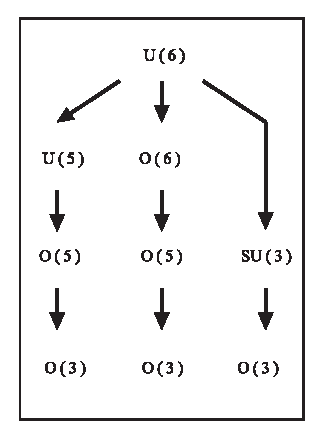
\includegraphics[scale=.65]{figure}
%
% If no graphics program available, insert a blank space i.e. use
%\picplace{5cm}{2cm} % Give the correct figure height and width in cm
%
\caption{Please write your figure caption here}
\label{fig:A1}       % Give a unique label
\end{figure}

% For tables use
%
\begin{table}
\caption{Please write your table caption here}
\label{tab:A1}       % Give a unique label
%
% Follow this input for your own table layout
%
\begin{tabular}{p{2cm}p{2.4cm}p{2cm}p{4.9cm}}
\hline\noalign{\smallskip}
Classes & Subclass & Length & Action Mechanism  \\
\noalign{\smallskip}\hline\noalign{\smallskip}
Translation & mRNA$^a$  & 22 (19--25) & Translation repression, mRNA cleavage\\
Translation & mRNA cleavage & 21 & mRNA cleavage\\
Translation & mRNA  & 21--22 & mRNA cleavage\\
Translation & mRNA  & 24--26 & Histone and DNA Modification\\
\noalign{\smallskip}\hline\noalign{\smallskip}
\end{tabular}
$^a$ Table foot note (with superscript)
\end{table}
%


%% -- Part-C
% !TEX root = ../../LN-Book.tex
%% -- Stand 2025/01/13
%% -- ulgr
%% -- Part C
%% --

\begin{partbacktext}
\part{Positive Semigroups on Banach Lattices}
\end{partbacktext}

\setcounter{chapter}{0}
%%%%%%%%%%%%%%%%%%%%%% chapter.tex %%%%%%%%%%%%%%%%%%%%%%%%%%%%%%%%%
%
% sample chapter
%
% Use this file as a template for your own input.
%
%%%%%%%%%%%%%%%%%%%%%%%% Springer-Verlag %%%%%%%%%%%%%%%%%%%%%%%%%%
%\motto{Use the template \emph{chapter.tex} to style the various elements of your chapter content.}
\chapter{Chapter Heading}
\label{intro} % Always give a unique label
% use \chaptermark{}
% to alter or adjust the chapter heading in the running head

\abstract*{Each chapter should be preceded by an abstract (no more than 200 words) that summarizes the content. The abstract will appear \textit{online} at \url{www.SpringerLink.com} and be available with unrestricted access. This allows unregistered users to read the abstract as a teaser for the complete chapter.
Please use the 'starred' version of the new \texttt{abstract} command for typesetting the text of the online abstracts (cf. source file of this chapter template \texttt{abstract}) and include them with the source files of your manuscript. Use the plain \texttt{abstract} command if the abstract is also to appear in the printed version of the book.}

\abstract{Each chapter should be preceded by an abstract (no more than 200 words) that summarizes the content. The abstract will appear \textit{online} at \url{www.SpringerLink.com} and be available with unrestricted access. This allows unregistered users to read the abstract as a teaser for the complete chapter. \newline\indent
Please use the 'starred' version of the new \texttt{abstract} command for typesetting the text of the online abstracts (cf. source file of this chapter template \texttt{abstract}) and include them with the source files of your manuscript. Use the plain \texttt{abstract} command if the abstract is also to appear in the printed version of the book.}

\section{Section Heading}
\label{sec:1}
Use the template \emph{chapter.tex} together with the document class SVMono (monograph-type books) or SVMult (edited books) to style the various elements of your chapter content conformable to the Springer Nature layout.

\section{Section Heading}
\label{sec:2}
% Always give a unique label
% and use \ref{<label>} for cross-references
% and \cite{<label>} for bibliographic references
% use \sectionmark{}
% to alter or adjust the section heading in the running head
Instead of simply listing headings of different levels we recommend to let every heading be followed by at least a short passage of text. Furtheron please use the \LaTeX\ automatism for all your cross-references and citations.

Please note that the first line of text that follows a heading is not indented, whereas the first lines of all subsequent paragraphs are.

\eject

Use the standard \verb|equation| environment to typeset your equations, e.g.
%
\begin{equation}
a \times b = c\;,
\end{equation}
%
however, for multiline equations we recommend to use the \verb|eqnarray| environment\footnote{In physics texts please activate the class option \texttt{vecphys} to depict your vectors in \textbf{\itshape boldface-italic} type - as is customary for a wide range of physical subjects.}.
\begin{eqnarray}
\left|\nabla U_{\alpha}^{\mu}(y)\right| &\le&\frac1{d-\alpha}\int
\left|\nabla\frac1{|\xi-y|^{d-\alpha}}\right|\,d\mu(\xi) =
\int \frac1{|\xi-y|^{d-\alpha+1}} \,d\mu(\xi)\qquad  \\
&=&(d-\alpha+1) \int\limits_{d(y)}^\infty
\frac{\mu(B(y,r))}{r^{d-\alpha+2}}\,dr \le (d-\alpha+1)
\int\limits_{d(y)}^\infty \frac{r^{d-\alpha}}{r^{d-\alpha+2}}\,dr
\label{eq:01}
\end{eqnarray}

\enlargethispage{24pt}

\subsection{Subsection Heading}
\label{subsec:2}
Instead of simply listing headings of different levels we recommend to let every heading be followed by at least a short passage of text. Further on please use the \LaTeX\ automatism for all your cross-references\index{cross-references} and citations\index{citations} as has already been described in Sect.~\ref{sec:2}.

\begin{quotation}
Please do not use quotation marks when quoting texts! Simply use the \verb|quotation| environment -- it will automatically be rendered in the preferred layout.
\end{quotation}


\subsubsection{Subsubsection Heading}
Instead of simply listing headings of different levels we recommend to let every heading be followed by at least a short passage of text. Furtheron please use the \LaTeX\ automatism for all your cross-references and citations as has already been described in Sect.~\ref{subsec:2}, see also Fig.~\ref{fig:1}\footnote{If you copy text passages, figures, or tables from other works, you must obtain \textit{permission} from the copyright holder (usually the original publisher). Please enclose the signed permission with the manucript. The sources\index{permission to print} must be acknowledged either in the captions, as footnotes or in a separate section of the book.}

Please note that the first line of text that follows a heading is not indented, whereas the first lines of all subsequent paragraphs are.

% For figures use
%
\begin{figure}[b]
\sidecaption
% Use the relevant command for your figure-insertion program
% to insert the figure file.
% For example, with the option graphics use
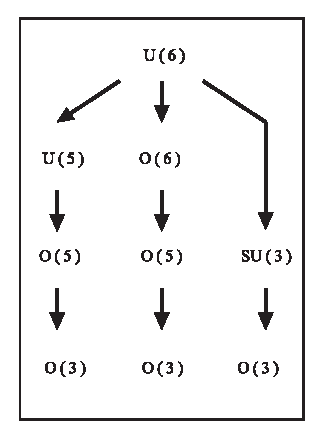
\includegraphics[scale=.65]{figure}
%
% If not, use
%\picplace{5cm}{2cm} % Give the correct figure height and width in cm
%
\caption{If the width of the figure is less than 7.8 cm use the \texttt{sidecapion} command to flush the caption on the left side of the page. If the figure is positioned at the top of the page, align the sidecaption with the top of the figure -- to achieve this you simply need to use the optional argument \texttt{[t]} with the \texttt{sidecaption} command}
\label{fig:1}       % Give a unique label
\end{figure}


\paragraph{Paragraph Heading} %
Instead of simply listing headings of different levels we recommend to let every heading be followed by at least a short passage of text. Furtheron please use the \LaTeX\ automatism for all your cross-references and citations as has already been described in Sect.~\ref{sec:2}.

Please note that the first line of text that follows a heading is not indented, whereas the first lines of all subsequent paragraphs are.

For typesetting numbered lists we recommend to use the \verb|enumerate| environment -- it will automatically render Springer's preferred layout.

\begin{enumerate}
\item{Livelihood and survival mobility are oftentimes coutcomes of uneven socioeconomic development.}
\begin{enumerate}
\item{Livelihood and survival mobility are oftentimes coutcomes of uneven socioeconomic development.}
\item{Livelihood and survival mobility are oftentimes coutcomes of uneven socioeconomic development.}
\end{enumerate}
\item{Livelihood and survival mobility are oftentimes coutcomes of uneven socioeconomic development.}
\end{enumerate}


\subparagraph{Subparagraph Heading} In order to avoid simply listing headings of different levels we recommend to let every heading be followed by at least a short passage of text. Use the \LaTeX\ automatism for all your cross-references and citations as has already been described in Sect.~\ref{sec:2}, see also Fig.~\ref{fig:2}.

Please note that the first line of text that follows a heading is not indented, whereas the first lines of all subsequent paragraphs are.

For unnumbered list we recommend to use the \verb|itemize| environment -- it will automatically render Springer's preferred layout.

\begin{itemize}
\item{Livelihood and survival mobility are oftentimes coutcomes of uneven socioeconomic development, cf. Table~\ref{tab:1}.}
\begin{itemize}
\item{Livelihood and survival mobility are oftentimes coutcomes of uneven socioeconomic development.}
\item{Livelihood and survival mobility are oftentimes coutcomes of uneven socioeconomic development.}
\end{itemize}
\item{Livelihood and survival mobility are oftentimes coutcomes of uneven socioeconomic development.}
\end{itemize}

\begin{figure}[t]
\sidecaption[t]
% Use the relevant command for your figure-insertion program
% to insert the figure file.
% For example, with the option graphics use
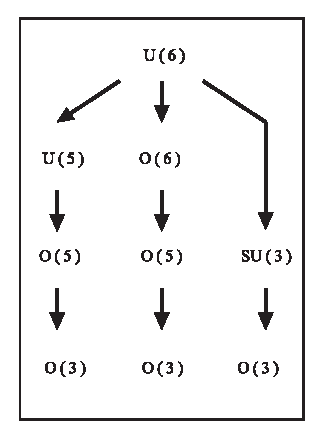
\includegraphics[scale=.65]{figure}
%
% If not, use
%\picplace{5cm}{2cm} % Give the correct figure height and width in cm
%
\caption{Please write your figure caption here}
\label{fig:2}       % Give a unique label
\end{figure}

\runinhead{Run-in Heading Boldface Version} Use the \LaTeX\ automatism for all your cross-references and citations as has already been described in Sect.~\ref{sec:2}.

\subruninhead{Run-in Heading Boldface and Italic Version} Use the \LaTeX\ automatism for all your cross-refer\-ences and citations as has already been described in Sect.~\ref{sec:2}\index{paragraph}.

\subsubruninhead{Run-in Heading Displayed Version} Use the \LaTeX\ automatism for all your cross-refer\-ences and citations as has already been described in Sect.~\ref{sec:2}\index{paragraph}.
% Use the \index{} command to code your index words
%
% For tables use
%
\begin{table}[!t]
\caption{Please write your table caption here}
\label{tab:1}       % Give a unique label
%
% For LaTeX tables use
%
\begin{tabular}{p{2cm}p{2.4cm}p{2cm}p{4.9cm}}
\hline\noalign{\smallskip}
Classes & Subclass & Length & Action Mechanism  \\
\noalign{\smallskip}\svhline\noalign{\smallskip}
Translation & mRNA$^a$  & 22 (19--25) & Translation repression, mRNA cleavage\\
Translation & mRNA cleavage & 21 & mRNA cleavage\\
Translation & mRNA  & 21--22 & mRNA cleavage\\
Translation & mRNA  & 24--26 & Histone and DNA Modification\\
\noalign{\smallskip}\hline\noalign{\smallskip}
\end{tabular}
$^a$ Table foot note (with superscript)
\end{table}
%
\section{Section Heading}
\label{sec:3}
% Always give a unique label
% and use \ref{<label>} for cross-references
% and \cite{<label>} for bibliographic references
% use \sectionmark{}
% to alter or adjust the section heading in the running head
Instead of simply listing headings of different levels we recommend to let every heading be followed by at least a short passage of text. Furtheron please use the \LaTeX\ automatism for all your cross-references and citations as has already been described in Sect.~\ref{sec:2}.

Please note that the first line of text that follows a heading is not indented, whereas the first lines of all subsequent paragraphs are.

If you want to list definitions or the like we recommend to use the Springer-enhanced \verb|description| environment -- it will automatically render Springer's preferred layout.

\begin{description}[Type 1]
\item[Type 1]{That addresses central themes pertainng to migration, health, and disease. In Sect.~\ref{sec:1}, Wilson discusses the role of human migration in infectious disease distributions and patterns.}
\item[Type 2]{That addresses central themes pertainng to migration, health, and disease. In Sect.~\ref{subsec:2}, Wilson discusses the role of human migration in infectious disease distributions and patterns.}
\end{description}

\subsection{Subsection Heading} %
In order to avoid simply listing headings of different levels we recommend to let every heading be followed by at least a short passage of text. Use the \LaTeX\ automatism for all your cross-references and citations citations as has already been described in Sect.~\ref{sec:2}.

Please note that the first line of text that follows a heading is not indented, whereas the first lines of all subsequent paragraphs are.

\begin{svgraybox}
If you want to emphasize complete paragraphs of texts we recommend to use the newly defined Springer class option \verb|graybox| and the newly defined environment \verb|svgraybox|. This will produce a 15 percent screened box 'behind' your text.

If you want to emphasize complete paragraphs of texts we recommend to use the newly defined Springer class option and environment \verb|svgraybox|. This will produce a 15 percent screened box 'behind' your text.
\end{svgraybox}


\subsubsection{Subsubsection Heading}
Instead of simply listing headings of different levels we recommend to let every heading be followed by at least a short passage of text. Furtheron please use the \LaTeX\ automatism for all your cross-references and citations as has already been described in Sect.~\ref{sec:2}.

Please note that the first line of text that follows a heading is not indented, whereas the first lines of all subsequent paragraphs are.

\begin{theorem}
Theorem text goes here.
\end{theorem}
%
% or
%
\begin{definition}
Definition text goes here.
\end{definition}

\begin{proof}
%\smartqed
Proof text goes here.
%\qed
\end{proof}

\paragraph{Paragraph Heading} %
Instead of simply listing headings of different levels we recommend to let every heading be followed by at least a short passage of text. Furtheron please use the \LaTeX\ automatism for all your cross-references and citations as has already been described in Sect.~\ref{sec:2}.

Note that the first line of text that follows a heading is not indented, whereas the first lines of all subsequent paragraphs are.
%
% For built-in environments use
%
\begin{theorem}
Theorem text goes here.
\end{theorem}
%
\begin{definition}
Definition text goes here.
\end{definition}
%
\begin{proof}
%\smartqed
Proof text goes here.
%\qed
\end{proof}
%
%
\begin{trailer}{Trailer Head}
If you want to emphasize complete paragraphs of texts in a \verb|Trailer Head| we recommend to
use  \begin{verbatim}\begin{trailer}{Trailer Head}
...
\end{trailer}\end{verbatim}
\end{trailer}
%
\begin{questype}{Questions}
If you want to emphasize complete paragraphs of texts in an \verb|Questions| we recommend to
use  \begin{verbatim}\begin{questype}{Questions}
...
\end{questype}\end{verbatim}
\end{questype}
%
%
\begin{important}{Important}
If you want to emphasize complete paragraphs of texts in an \verb|Important| we recommend to
use  \begin{verbatim}\begin{important}{Important}
...
\end{important}\end{verbatim}
\end{important}
%
\clearpage
\begin{warning}{Attention}
If you want to emphasize complete paragraphs of texts in an \verb|Attention| we recommend to
use  \begin{verbatim}\begin{warning}{Attention}
...
\end{warning}\end{verbatim}
\end{warning}

\begin{programcode}{Program Code}
If you want to emphasize complete paragraphs of texts in a \verb|Program Code| we recommend to
use

\verb|\begin{programcode}{Program Code}|

\verb|\begin{verbatim}...\end{verbatim}|

\verb|\end{programcode}|

\end{programcode}
%
\begin{tips}{Tips}
If you want to emphasize complete paragraphs of texts in a \verb|Tips| we recommend to
use  \begin{verbatim}\begin{tips}{Tips}
...
\end{tips}\end{verbatim}
\end{tips}
%
%
\begin{overview}{Overview}
If you want to emphasize complete paragraphs of texts in an \verb|Overview| we recommend to
use  \begin{verbatim}\begin{overview}{Overview}
...
\end{overview}\end{verbatim}
\end{overview}
\clearpage
\begin{backgroundinformation}{Background Information}
If you want to emphasize complete paragraphs of texts in a \verb|Background|
\verb|Information| we recommend to
use

\verb|\begin{backgroundinformation}{Background Information}|

\verb|...|

\verb|\end{backgroundinformation}|
\end{backgroundinformation}
\begin{legaltext}{Legal Text}
If you want to emphasize complete paragraphs of texts in a \verb|Legal Text| we recommend to
use  \begin{verbatim}\begin{legaltext}{Legal Text}
...
\end{legaltext}\end{verbatim}
\end{legaltext}
%
\begin{acknowledgement}
If you want to include acknowledgments of assistance and the like at the end of an individual chapter please use the \verb|acknowledgement| environment -- it will automatically render Springer's preferred layout.
\end{acknowledgement}
%
\section*{Appendix}
\addcontentsline{toc}{section}{Appendix}
%
When placed at the end of a chapter or contribution (as opposed to at the end of the book), the numbering of tables, figures, and equations in the appendix section continues on from that in the main text. Hence please \textit{do not} use the \verb|appendix| command when writing an appendix at the end of your chapter or contribution. If there is only one the appendix is designated ``Appendix'', or ``Appendix 1'', or ``Appendix 2'', etc. if there is more than one.

\begin{equation}
a \times b = c
\end{equation}
% Problems or Exercises should be sorted chapterwise
\section*{Problems}
\addcontentsline{toc}{section}{Problems}
%
% Use the following environment.
% Don't forget to label each problem;
% the label is needed for the solutions' environment
\begin{prob}
\label{prob1}
A given problem or Excercise is described here. The
problem is described here. The problem is described here.
\end{prob}

\begin{prob}
\label{prob2}
\textbf{Problem Heading}\\
(a) The first part of the problem is described here.\\
(b) The second part of the problem is described here.
\end{prob}

%%%%%%%%%%%%%%%%%%%%%%%% referenc.tex %%%%%%%%%%%%%%%%%%%%%%%%%%%%%%
% sample references
% %
% Use this file as a template for your own input.
%
%%%%%%%%%%%%%%%%%%%%%%%% Springer-Verlag %%%%%%%%%%%%%%%%%%%%%%%%%%
%
% BibTeX users please use
% \bibliographystyle{}
% \bibliography{}
%
%\biblstarthook{
\section{Styling of References}
In view of the parallel print and (chapter-wise) online publication of your book at \url{www.springerlink.com} it has been decided that -- as a genreral rule --  references should be sorted chapter-wise and placed at the end of the individual chapters. However, upon agreement with your contact at Springer you may list your references in a single seperate chapter at the end of your book. Deactivate the class option \texttt{sectrefs} and the \texttt{thebibliography} environment will be put out as a chapter of its own.\\\indent
References may be \textit{cited} in the text either by number (preferred) or by author/year.\footnote{Make sure that all references from the list are cited in the text. Those not cited should be moved to a separate \textit{Further Reading} section or chapter.} If the citatiion in the text is numbered, the reference list should be arranged in ascending order. If the citation in the text is author/year, the reference list should be \textit{sorted} alphabetically and if there are several works by the same author, the following order should be used:
\begin{enumerate}
\item all works by the author alone, ordered chronologically by year of publication
\item all works by the author with a coauthor, ordered alphabetically by coauthor
\item all works by the author with several coauthors, ordered chronologically by year of publication.
\end{enumerate}
The \textit{styling} of references\footnote{Always use the standard abbreviation of a journal's name according to the ISSN \textit{List of Title Word Abbreviations}, see \url{http://www.issn.org/en/node/344}} depends on the subject of your book:
\begin{itemize}
\item The \textit{two} recommended styles for references in books on \textit{mathematical, physical, statistical and computer sciences} are depicted in ~\cite{science-contrib, science-online, science-mono, science-journal, science-DOI} and ~\cite{phys-online, phys-mono, phys-journal, phys-DOI, phys-contrib}.
\item Examples of the most commonly used reference style in books on \textit{Psychology, Social Sciences} are~\cite{psysoc-mono, psysoc-online,psysoc-journal, psysoc-contrib, psysoc-DOI}.
\item Examples for references in books on \textit{Humanities, Linguistics, Philosophy} are~\cite{humlinphil-journal, humlinphil-contrib, humlinphil-mono, humlinphil-online, humlinphil-DOI}.
\item Examples of the basic Springer style used in publications on a wide range of subjects such as \textit{Computer Science, Economics, Engineering, Geosciences, Life Sciences, Medicine, Biomedicine} are ~\cite{basic-contrib, basic-online, basic-journal, basic-DOI, basic-mono}. 
\end{itemize}
%}

\begin{thebibliography}{99.}%
% and use \bibitem to create references.
%
% Use the following syntax and markup for your references if 
% the subject of your book is from the field 
% "Mathematics, Physics, Statistics, Computer Science"
%
% Contribution 
\bibitem{science-contrib} Broy, M.: Software engineering --- from auxiliary to key technologies. In: Broy, M., Dener, E. (eds.) Software Pioneers, pp. 10-13. Springer, Heidelberg (2002)
%
% Online Document
\bibitem{science-online} Dod, J.: Effective substances. In: The Dictionary of Substances and Their Effects. Royal Society of Chemistry (1999) Available via DIALOG. \\
\url{http://www.rsc.org/dose/title of subordinate document. Cited 15 Jan 1999}
%
% Monograph
\bibitem{science-mono} Geddes, K.O., Czapor, S.R., Labahn, G.: Algorithms for Computer Algebra. Kluwer, Boston (1992) 
%
% Journal article
\bibitem{science-journal} Hamburger, C.: Quasimonotonicity, regularity and duality for nonlinear systems of partial differential equations. Ann. Mat. Pura. Appl. \textbf{169}, 321--354 (1995)
%
% Journal article by DOI
\bibitem{science-DOI} Slifka, M.K., Whitton, J.L.: Clinical implications of dysregulated cytokine production. J. Mol. Med. (2000) doi: 10.1007/s001090000086 
%
%\bigskip

% Use the following (APS) syntax and markup for your references if 
% the subject of your book is from the field 
% "Mathematics, Physics, Statistics, Computer Science"
%
% Online Document
\bibitem{phys-online} J. Dod, in \textit{The Dictionary of Substances and Their Effects}, Royal Society of Chemistry. (Available via DIALOG, 1999), 
\url{http://www.rsc.org/dose/title of subordinate document. Cited 15 Jan 1999}
%
% Monograph
\bibitem{phys-mono} H. Ibach, H. L\"uth, \textit{Solid-State Physics}, 2nd edn. (Springer, New York, 1996), pp. 45-56 
%
% Journal article
\bibitem{phys-journal} S. Preuss, A. Demchuk Jr., M. Stuke, Appl. Phys. A \textbf{61}
%
% Journal article by DOI
\bibitem{phys-DOI} M.K. Slifka, J.L. Whitton, J. Mol. Med., doi: 10.1007/s001090000086
%
% Contribution 
\bibitem{phys-contrib} S.E. Smith, in \textit{Neuromuscular Junction}, ed. by E. Zaimis. Handbook of Experimental Pharmacology, vol 42 (Springer, Heidelberg, 1976), p. 593
%
%\bigskip
%
% Use the following syntax and markup for your references if 
% the subject of your book is from the field 
% "Psychology, Social Sciences"
%
%
% Monograph
\bibitem{psysoc-mono} Calfee, R.~C., \& Valencia, R.~R. (1991). \textit{APA guide to preparing manuscripts for journal publication.} Washington, DC: American Psychological Association.
%
% Online Document
\bibitem{psysoc-online} Dod, J. (1999). Effective substances. In: The dictionary of substances and their effects. Royal Society of Chemistry. Available via DIALOG. \\
\url{http://www.rsc.org/dose/Effective substances.} Cited 15 Jan 1999.
%
% Journal article
\bibitem{psysoc-journal} Harris, M., Karper, E., Stacks, G., Hoffman, D., DeNiro, R., Cruz, P., et al. (2001). Writing labs and the Hollywood connection. \textit{J Film} Writing, 44(3), 213--245.
%
% Contribution 
\bibitem{psysoc-contrib} O'Neil, J.~M., \& Egan, J. (1992). Men's and women's gender role journeys: Metaphor for healing, transition, and transformation. In B.~R. Wainrig (Ed.), \textit{Gender issues across the life cycle} (pp. 107--123). New York: Springer.
%
% Journal article by DOI
\bibitem{psysoc-DOI}Kreger, M., Brindis, C.D., Manuel, D.M., Sassoubre, L. (2007). Lessons learned in systems change initiatives: benchmarks and indicators. \textit{American Journal of Community Psychology}, doi: 10.1007/s10464-007-9108-14.
%
%
% Use the following syntax and markup for your references if 
% the subject of your book is from the field 
% "Humanities, Linguistics, Philosophy"
%
%\bigskip
%
% Journal article
\bibitem{humlinphil-journal} Alber John, Daniel C. O'Connell, and Sabine Kowal. 2002. Personal perspective in TV interviews. \textit{Pragmatics} 12:257--271
%
% Contribution 
\bibitem{humlinphil-contrib} Cameron, Deborah. 1997. Theoretical debates in feminist linguistics: Questions of sex and gender. In \textit{Gender and discourse}, ed. Ruth Wodak, 99--119. London: Sage Publications.
%
% Monograph
\bibitem{humlinphil-mono} Cameron, Deborah. 1985. \textit{Feminism and linguistic theory.} New York: St. Martin's Press.
%
% Online Document
\bibitem{humlinphil-online} Dod, Jake. 1999. Effective substances. In: The dictionary of substances and their effects. Royal Society of Chemistry. Available via DIALOG. \\
http://www.rsc.org/dose/title of subordinate document. Cited 15 Jan 1999
%
% Journal article by DOI
\bibitem{humlinphil-DOI} Suleiman, Camelia, Daniel C. O'Connell, and Sabine Kowal. 2002. `If you and I, if we, in this later day, lose that sacred fire...': Perspective in political interviews. \textit{Journal of Psycholinguistic Research}. doi: 10.1023/A:1015592129296.
%
%
%
%\bigskip
%
%
% Use the following syntax and markup for your references if 
% the subject of your book is from the field 
% "Computer Science, Economics, Engineering, Geosciences, Life Sciences"
%
%
% Contribution 
\bibitem{basic-contrib} Brown B, Aaron M (2001) The politics of nature. In: Smith J (ed) The rise of modern genomics, 3rd edn. Wiley, New York 
%
% Online Document
\bibitem{basic-online} Dod J (1999) Effective Substances. In: The dictionary of substances and their effects. Royal Society of Chemistry. Available via DIALOG. \\
\url{http://www.rsc.org/dose/title of subordinate document. Cited 15 Jan 1999}
%
% Journal article by DOI
\bibitem{basic-DOI} Slifka MK, Whitton JL (2000) Clinical implications of dysregulated cytokine production. J Mol Med, doi: 10.1007/s001090000086
%
% Journal article
\bibitem{basic-journal} Smith J, Jones M Jr, Houghton L et al (1999) Future of health insurance. N Engl J Med 965:325--329
%
% Monograph
\bibitem{basic-mono} South J, Blass B (2001) The future of modern genomics. Blackwell, London 
%
\end{thebibliography}


%%%%%%%%%%%%%%%%%%%%%% appendix.tex %%%%%%%%%%%%%%%%%%%%%%%%%%%%%%%%%
%
% sample appendix
%
% Use this file as a template for your own input.
%
%%%%%%%%%%%%%%%%%%%%%%%% Springer-Verlag %%%%%%%%%%%%%%%%%%%%%%%%%%

\chapter{Chapter Heading}
\label{introA} % Always give a unique label
% use \chaptermark{}
% to alter or adjust the chapter heading in the running head

Use the template \emph{appendix.tex} together with the document class SVMono (monograph-type books) or SVMult (edited books) to style appendix of your book.


\section{Section Heading}
\label{sec:A1}
% Always give a unique label
% and use \ref{<label>} for cross-references
% and \cite{<label>} for bibliographic references
% use \sectionmark{}
% to alter or adjust the section heading in the running head
Instead of simply listing headings of different levels we recommend to let every heading be followed by at least a short passage of text. Further on please use the \LaTeX\ automatism for all your cross-references and citations.


\subsection{Subsection Heading}
\label{sec:A2}
Instead of simply listing headings of different levels we recommend to let every heading be followed by at least a short passage of text. Further on please use the \LaTeX\ automatism for all your cross-references and citations as has already been described in Sect.~\ref{sec:A1}.

For multiline equations we recommend to use the \verb|eqnarray| environment.
\begin{eqnarray}
\vec{a}\times\vec{b}=\vec{c} \nonumber\\
\vec{a}\times\vec{b}=\vec{c}
\label{eq:A01}
\end{eqnarray}

\subsubsection{Subsubsection Heading}
Instead of simply listing headings of different levels we recommend to let every heading be followed by at least a short passage of text. Further on please use the \LaTeX\ automatism for all your cross-references and citations as has already been described in Sect.~\ref{sec:A2}.

Please note that the first line of text that follows a heading is not indented, whereas the first lines of all subsequent paragraphs are.

% For figures use
%
\begin{figure}[t]
\sidecaption[t]
% Use the relevant command for your figure-insertion program
% to insert the figure file.
% For example, with the graphicx style use
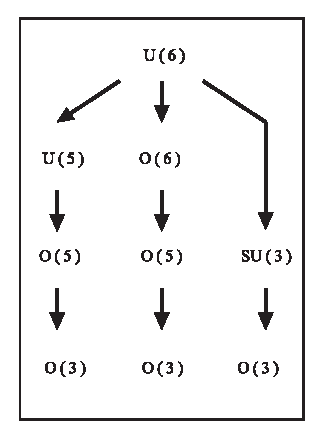
\includegraphics[scale=.65]{figure}
%
% If no graphics program available, insert a blank space i.e. use
%\picplace{5cm}{2cm} % Give the correct figure height and width in cm
%
\caption{Please write your figure caption here}
\label{fig:A1}       % Give a unique label
\end{figure}

% For tables use
%
\begin{table}
\caption{Please write your table caption here}
\label{tab:A1}       % Give a unique label
%
% Follow this input for your own table layout
%
\begin{tabular}{p{2cm}p{2.4cm}p{2cm}p{4.9cm}}
\hline\noalign{\smallskip}
Classes & Subclass & Length & Action Mechanism  \\
\noalign{\smallskip}\hline\noalign{\smallskip}
Translation & mRNA$^a$  & 22 (19--25) & Translation repression, mRNA cleavage\\
Translation & mRNA cleavage & 21 & mRNA cleavage\\
Translation & mRNA  & 21--22 & mRNA cleavage\\
Translation & mRNA  & 24--26 & Histone and DNA Modification\\
\noalign{\smallskip}\hline\noalign{\smallskip}
\end{tabular}
$^a$ Table foot note (with superscript)
\end{table}
%


%% -- Part-D
%%%%%%%%%%%%%%%%%%%%%part.tex%%%%%%%%%%%%%%%%%%%%%%%%%%%%%%%%%%
% 
% Part D
%
%
%%%%%%%%%%%%%%%%%%%%%%%% Springer %%%%%%%%%%%%%%%%%%%%%%%%%%

\begin{partbacktext}
\part[Positive Semigroups on $C^{*}$- and $W^{*}$-Algebras]{Positive Semigroups on \\$C^{*}$- and $W^{*}$-Algebras}
\end{partbacktext}
% !TEX root = ../../LN-Book.tex
%% -- Stand 2025/01/17
%% -- ulgr
%% -- Part D1
%% --
\chapter{Basic Results}% on Semigroups and Operator Algebras}
%% --
This is not a systematic introduction into the theory of strongly continuous semigroups on $\mathrm{C}^{*}$ and \WA-algebras.
For that we refer to Bratteli-Robinson (1979), Davies (1976) and the survey article of Oseledets (1984).
We only prepare for the subsequent chapters on spectral theory and asymptotics by fixing the notations and introducing some standard constructions.
%% --
\section{Notations}
%% --
1. By $M$ we shall denote a $C^{*}$-algebra with unit 1.
$M^{\text{sa}} := \{x \in M : x^{*} = x\}$ is the selfadjoint part of $M$ and $M_{+} := \{x^{*} x : x \in M\}$ the positive cone in $M$.
If $M'$ is the dual of $M$, then $M'_{+} = \{\psi \in M' : \psi(x) \geq 0, x \in M_{+}\}$ is a weak*-closed generating cone in $M'$.
$S(M) := \{\psi \in M'_{+} : \psi(1) = 1\}$ is called the state space of $M$.
For the theory of $C^{*}$-algebras and related notions we refer to [Pedersen (1979)].
$M$ is called a $W^{*}$-algebra, if there exists a Banach space $M_{*}$, such that its dual $(M_{*})^{'}$ is (isomorphic to) $M$.
We call $M_{*}$ the predual of $M$ and $\psi \in M_{*}$ a normal linear functional.
It is known that $M_{*}$ is unique [Sakai (1971), 1.13.3.].
For further properties of $M_{*}$ we refer to [Takesaki (1979), Chapter III].

\smallskip
\noindent2. A map $T \in L(M)$ is called positive (in symbols $T \geq 0$) if $T(M_{+}) \leq M_{+}$.
$T \in L(M)$ is called $n$-positive ($n \in \mathbb{N}$) if $T \otimes id_n$ is positive from $M \otimes M_n$ in $M \otimes M_n$, where $id_n$ is the identity map on the $C^{*}$-algebra $M_n$ of all $n \times n$-matrices.
Obviously, every $n$-positive map is positive.
We call $T \in L(M)$ a Schwarz map if $T$ satisfies the inequality
\[
T(x)T(x)^{*} \leq T(xx^{*}), x \in M
\]
Note that such $T$ is necessarily a contraction.
It is well known that every $n$-positive contraction, $n \geq 2$ and that every positive contraction on a commutative $C^{*}$-algebra is a Schwarz map [Takesaki (1979), Corollary IV.3.8.].
As we shall see, the Schwarz inequality is crucial for our investigations.

\smallskip
\noindent3. If $M$ is a $C^{*}$-algebra we assume $T = (T(t))_{t \geq 0}$ to be a strongly continuous semigroup (abbreviated semigroup) while on $W^{*}$-algebras we consider weak*-semigroups, i.e. the mapping $(t \rightarrow T(t)x)$ is continuous from $\mathbb{R}_{+}$ into $(M, \sigma(M, M_{*}))$, $M_{*}$ the predual of $M$, and every $T(t) \in T$ is $\sigma(M, M_{*})$-continuous.
Note that the preadjoint semigroup
\[
T_{*} = \{T(t)_{*} : T(t) \in T\}
\]
is weakly, hence strongly continuous on $M_{*}$ (see e.g., Davies (1980), Prop.1.23).
We call $T$ identity preserving if $T(t)1 = 1$ and of Schwarz type if every $T(t) \in T$ is a Schwarz map.
For the notations concerning one-parameter semigroups we refer to part A.
In addition we recommend to compare the results of this section of the book with the corresponding results for commutative $C^{*}$-algebras, i.e. for $C_0(X)$, $C(K)$ and $L^\infty(\mu)$ (see Part B).

\section{A Fundamental Inequality for the Resolvent}

If $T=(T(t))_{t \geq 0}$ is a strongly continuous semigroup of Schwarz maps on a $C^{*}$-algebra $M$ (resp. a weak*-semigroup of Schwarz type on a $W^{*}$-algebra $M$) with generator $A$, then the spectral bound $s(A) \leq 0$.
Then for $\lambda \in \mathbb{C}$, $\operatorname{Re}(\lambda)>0$, there exists a representation for the resolvent $R(\lambda, A)$ given by the formula
\[
R(\lambda, A)x = \int_{0}^{\infty} e^{-\lambda t} T(t)x dt, \quad x \in M
\]
where the integral exists in the norm topology.

In [Bratteli-Robinson (1979)] it is shown that $T$ is a semigroup of Schwarz type if and only if $R(\mu, A)$ is a Schwarz map for every $\mu \in \mathbb{R}_{+}$.
Here we relate the domination of two semigroups to an inequality for the corresponding resolvent operator.
This inequality will be needed later.
%$% -- 
\begin{theorem}
Let $T=(T(t))_{t \geq 0}$ be a semigroup of Schwarz type and $S=(S(t))_{t \geq 0}$ a semigroup on a $C^{*}$-algebra $M$ with generators $A$ and $B$, respectively.
If 
\[
(S(t)x)(S(t)x)^{*} \leq T(t)xx^{*}
\]
for all $x \in M$ and $t \in \mathbb{R}_{+}$, then
\[
(\mu R(\mu, B)x)(\mu R(\mu, B)x)^{*} \leq \mu R(\mu, A)xx^{*}
\]
for all $x \in M$ and $\mu \in \mathbb{R}_{+}$.
The same result holds if $T$ is a weak*-semigroup of Schwarz type and $S$ is a weak*-semigroup on a $W^{*}$-algebra $M$ such that (*) is fulfilled.
\end{theorem}
%% --
\begin{proof}
From the assumption (*) it follows that
\begin{align*}
0 &\leq (S(r)x - S(t)x)(S(r)x - S(t)x)^{*} \\
&= (S(r)x)(S(r)x)^{*} - (S(r)x)(S(t)x)^{*} - (S(t)x)(S(r)x)^{*} + (S(t)x)(S(t)x)^{*} \\
&\leq T(r)xx^{*} + T(t)xx^{*} - (S(r)x)(S(t)x)^{*} - (S(t)x)(S(r)x)^{*}
\end{align*}
for every $r,t \in \mathbb{R}_{+}$.
Hence
%% --
\[
(S(r)x)(S(t)x)^{*} + (S(t)x)(S(r)x)^{*} \leq T(r)xx^{*} + T(t)xx^{*}
\]
%% --
Obviously, $\|S(t)\| \leq 1$ for all $t \in \mathbb{R}_{+}$.
Then for all $\mu \in \mathbb{R}_{+}$ and $x \in M$:
%% --
\begin{align*}
&(R(\mu, B)x)(R(\mu, B)x)^{*} \\
&= \left(\int_{0}^{\infty} e^{-\mu r} S(r)x dr\right)\left(\int_{0}^{\infty} e^{-\mu t} S(t)x dt\right)^{*} \\
&= \frac{1}{2}\left(\int_{0}^{\infty} \int_{0}^{\infty} e^{-\mu(r+t)}((S(r)x)(S(t)x)^{*} + (S(t)x)(S(r)x)^{*}) dr dt\right) \\
&\leq \frac{1}{2}\left(\int_{0}^{\infty} \int_{0}^{\infty} e^{-\mu(r+t)}(T(r)xx^{*} + T(t)xx^{*}) dr dt\right) \\
&= \left(\int_{0}^{\infty} e^{-\mu s} ds\right)\left(\int_{0}^{\infty} e^{-\mu t} T(t)xx^{*} dt\right) = \mu^{-1} R(\mu, A)xx^{*}
\end{align*}
where the handling of the integral is justified by [Bourbaki (1955), §8, $n^{\circ}$ 4, Proposition 9].
\end{proof}

\begin{corollary} 
Let $T$ be a semigroup of Schwarz maps (resp., weak*-semigroup of Schwarz maps).
Then for all $\lambda \in \mathbb{C}$ with $\operatorname{Re}(\lambda)>0$:
\[
(R(\lambda, A)x)(R(\lambda, A)x)^{*} \leq (\operatorname{Re}\lambda)^{-1} R(\operatorname{Re}\lambda, A)xx^{*}, \quad x \in M
\]
In particular for all $(\mu, \alpha) \in \mathbb{R}_{+} \times \mathbb{R}, x \in M$:
\[
(\mu R(\mu+i\alpha, A)x)(\mu R(\mu+i\alpha, A)x)^{*} \leq \mu R(\mu, A)(xx^{*})
\]
\end{corollary}
%% --
\begin{proof}
Let $\lambda \in \mathbb{C}$ with $\operatorname{Re}(\lambda)>0$.
Then the semigroup
\[
S := (e^{-i\operatorname{Im}(\lambda)t}T(t))_{t \geq 0}
\]
fulfils the assumption of Thm 2.1. and $B := A-i\lambda$ is the generator of $S$.
Consequently $R(\lambda, A)=R(\operatorname{Re}\lambda, B)$ and the corollary follows from Theorem 2.1.
\end{proof}
%% --
As in section C-III the following notion will be an important tool for the spectral theory of semigroups.
%% --
\begin{definition} 
Let $E$ be a Banach space and $\emptyset \neq D$ an open subset of $\mathbb{C}$.
A family $R: D \rightarrow L(E)$ is called a pseudo-resolvent on $D$ with values in $E$ if
%% --
\[
R(\lambda)-R(\mu)=-(\lambda-\mu)R(\lambda)R(\mu)
\]
for all $\lambda$ and $\mu$ in $D$.
%% --
If $R$ is a pseudo-resolvent on $D=\{\lambda \in \mathbb{C}: \operatorname{Re}(\lambda) > 0\}$ with values in a $C^{*}$- or $W^{*}$-algebra, then $R$ is called of Schwarz type if
%% --
\[
(R(\lambda)x)(R(\lambda)x)^{*} \leq (\operatorname{Re}\lambda)^{-1}R(\operatorname{Re}\lambda)xx^{*}
\]
%% --
for all $\lambda \in D$ and $x \in M$.
$R$ is called identity preserving if $\lambda R(\lambda)1 = 1$ for all $\lambda \in D$.
\end{definition}
%% --
For examples and properties of a pseudo-resolvent see C-III, 2.5.
We state what will be used without further reference.
%% --
\begin{enumerate}
\item
If $a \in \mathbb{C}$ and $x \in E$ such that $(a-\lambda)R(\lambda)x = x$ for some $\lambda \in D$, then $(a-\mu)R(\mu)x = x$ for all $\mu \in D$ (use the \enquote{resolvent equation}).

\item
If $F$ is a closed subspace of $E$ such that $R(\lambda)F \subseteq F$ for some $\lambda \in D$, then $R(\mu)F \subseteq F$ for all $\mu$ in a neighbourhood of $\lambda$.
This follows from the fact that for all $\mu \in D$ near $\lambda$ the pseudo-resolvent in $\mu$ is given by
%% --
\[
R(\mu) = \sum_{n}(\lambda-\mu)^n R(\lambda)^{n+1}
\]
%% --
\end{enumerate}
%% --
\begin{definition} 
We call a semigroup $T$ on the predual $M_{*}$ of a $W^{*}$-algebra $M$ identity preserving and of Schwarz type, if its adjoint weak*-semigroup has these properties.
Likewise, a pseudo-resolvent $R$ on $D=\{\lambda \in \mathbb{C}: \operatorname{Re}(\lambda)>0\}$ with values in $M_{*}$ is called identity preserving and of Schwarz type, if $R'$ has these properties.
\end{definition}
%% --
%%%%%%%%%%%%%%%%%%%%%% appendix.tex %%%%%%%%%%%%%%%%%%%%%%%%%%%%%%%%%
%
% sample appendix
%
% Use this file as a template for your own input.
%
%%%%%%%%%%%%%%%%%%%%%%%% Springer-Verlag %%%%%%%%%%%%%%%%%%%%%%%%%%

\chapter{Chapter Heading}
\label{introA} % Always give a unique label
% use \chaptermark{}
% to alter or adjust the chapter heading in the running head

Use the template \emph{appendix.tex} together with the document class SVMono (monograph-type books) or SVMult (edited books) to style appendix of your book.


\section{Section Heading}
\label{sec:A1}
% Always give a unique label
% and use \ref{<label>} for cross-references
% and \cite{<label>} for bibliographic references
% use \sectionmark{}
% to alter or adjust the section heading in the running head
Instead of simply listing headings of different levels we recommend to let every heading be followed by at least a short passage of text. Further on please use the \LaTeX\ automatism for all your cross-references and citations.


\subsection{Subsection Heading}
\label{sec:A2}
Instead of simply listing headings of different levels we recommend to let every heading be followed by at least a short passage of text. Further on please use the \LaTeX\ automatism for all your cross-references and citations as has already been described in Sect.~\ref{sec:A1}.

For multiline equations we recommend to use the \verb|eqnarray| environment.
\begin{eqnarray}
\vec{a}\times\vec{b}=\vec{c} \nonumber\\
\vec{a}\times\vec{b}=\vec{c}
\label{eq:A01}
\end{eqnarray}

\subsubsection{Subsubsection Heading}
Instead of simply listing headings of different levels we recommend to let every heading be followed by at least a short passage of text. Further on please use the \LaTeX\ automatism for all your cross-references and citations as has already been described in Sect.~\ref{sec:A2}.

Please note that the first line of text that follows a heading is not indented, whereas the first lines of all subsequent paragraphs are.

% For figures use
%
\begin{figure}[t]
\sidecaption[t]
% Use the relevant command for your figure-insertion program
% to insert the figure file.
% For example, with the graphicx style use
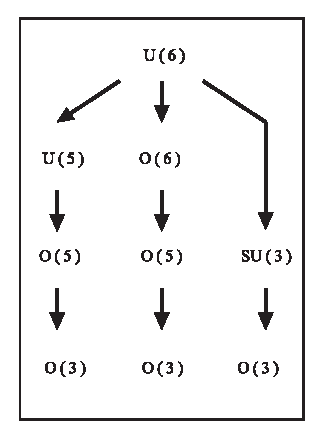
\includegraphics[scale=.65]{figure}
%
% If no graphics program available, insert a blank space i.e. use
%\picplace{5cm}{2cm} % Give the correct figure height and width in cm
%
\caption{Please write your figure caption here}
\label{fig:A1}       % Give a unique label
\end{figure}

% For tables use
%
\begin{table}
\caption{Please write your table caption here}
\label{tab:A1}       % Give a unique label
%
% Follow this input for your own table layout
%
\begin{tabular}{p{2cm}p{2.4cm}p{2cm}p{4.9cm}}
\hline\noalign{\smallskip}
Classes & Subclass & Length & Action Mechanism  \\
\noalign{\smallskip}\hline\noalign{\smallskip}
Translation & mRNA$^a$  & 22 (19--25) & Translation repression, mRNA cleavage\\
Translation & mRNA cleavage & 21 & mRNA cleavage\\
Translation & mRNA  & 21--22 & mRNA cleavage\\
Translation & mRNA  & 24--26 & Histone and DNA Modification\\
\noalign{\smallskip}\hline\noalign{\smallskip}
\end{tabular}
$^a$ Table foot note (with superscript)
\end{table}
%


%% -- Part-E
%\include{author/part-a/ln-part-e}
%%%%%%%%%%%%%%%%%%%%%% chapter.tex %%%%%%%%%%%%%%%%%%%%%%%%%%%%%%%%%
%
% sample chapter
%
% Use this file as a template for your own input.
%
%%%%%%%%%%%%%%%%%%%%%%%% Springer-Verlag %%%%%%%%%%%%%%%%%%%%%%%%%%
%\motto{Use the template \emph{chapter.tex} to style the various elements of your chapter content.}
\chapter{Chapter Heading}
\label{intro} % Always give a unique label
% use \chaptermark{}
% to alter or adjust the chapter heading in the running head

\abstract*{Each chapter should be preceded by an abstract (no more than 200 words) that summarizes the content. The abstract will appear \textit{online} at \url{www.SpringerLink.com} and be available with unrestricted access. This allows unregistered users to read the abstract as a teaser for the complete chapter.
Please use the 'starred' version of the new \texttt{abstract} command for typesetting the text of the online abstracts (cf. source file of this chapter template \texttt{abstract}) and include them with the source files of your manuscript. Use the plain \texttt{abstract} command if the abstract is also to appear in the printed version of the book.}

\abstract{Each chapter should be preceded by an abstract (no more than 200 words) that summarizes the content. The abstract will appear \textit{online} at \url{www.SpringerLink.com} and be available with unrestricted access. This allows unregistered users to read the abstract as a teaser for the complete chapter. \newline\indent
Please use the 'starred' version of the new \texttt{abstract} command for typesetting the text of the online abstracts (cf. source file of this chapter template \texttt{abstract}) and include them with the source files of your manuscript. Use the plain \texttt{abstract} command if the abstract is also to appear in the printed version of the book.}

\section{Section Heading}
\label{sec:1}
Use the template \emph{chapter.tex} together with the document class SVMono (monograph-type books) or SVMult (edited books) to style the various elements of your chapter content conformable to the Springer Nature layout.

\section{Section Heading}
\label{sec:2}
% Always give a unique label
% and use \ref{<label>} for cross-references
% and \cite{<label>} for bibliographic references
% use \sectionmark{}
% to alter or adjust the section heading in the running head
Instead of simply listing headings of different levels we recommend to let every heading be followed by at least a short passage of text. Furtheron please use the \LaTeX\ automatism for all your cross-references and citations.

Please note that the first line of text that follows a heading is not indented, whereas the first lines of all subsequent paragraphs are.

\eject

Use the standard \verb|equation| environment to typeset your equations, e.g.
%
\begin{equation}
a \times b = c\;,
\end{equation}
%
however, for multiline equations we recommend to use the \verb|eqnarray| environment\footnote{In physics texts please activate the class option \texttt{vecphys} to depict your vectors in \textbf{\itshape boldface-italic} type - as is customary for a wide range of physical subjects.}.
\begin{eqnarray}
\left|\nabla U_{\alpha}^{\mu}(y)\right| &\le&\frac1{d-\alpha}\int
\left|\nabla\frac1{|\xi-y|^{d-\alpha}}\right|\,d\mu(\xi) =
\int \frac1{|\xi-y|^{d-\alpha+1}} \,d\mu(\xi)\qquad  \\
&=&(d-\alpha+1) \int\limits_{d(y)}^\infty
\frac{\mu(B(y,r))}{r^{d-\alpha+2}}\,dr \le (d-\alpha+1)
\int\limits_{d(y)}^\infty \frac{r^{d-\alpha}}{r^{d-\alpha+2}}\,dr
\label{eq:01}
\end{eqnarray}

\enlargethispage{24pt}

\subsection{Subsection Heading}
\label{subsec:2}
Instead of simply listing headings of different levels we recommend to let every heading be followed by at least a short passage of text. Further on please use the \LaTeX\ automatism for all your cross-references\index{cross-references} and citations\index{citations} as has already been described in Sect.~\ref{sec:2}.

\begin{quotation}
Please do not use quotation marks when quoting texts! Simply use the \verb|quotation| environment -- it will automatically be rendered in the preferred layout.
\end{quotation}


\subsubsection{Subsubsection Heading}
Instead of simply listing headings of different levels we recommend to let every heading be followed by at least a short passage of text. Furtheron please use the \LaTeX\ automatism for all your cross-references and citations as has already been described in Sect.~\ref{subsec:2}, see also Fig.~\ref{fig:1}\footnote{If you copy text passages, figures, or tables from other works, you must obtain \textit{permission} from the copyright holder (usually the original publisher). Please enclose the signed permission with the manucript. The sources\index{permission to print} must be acknowledged either in the captions, as footnotes or in a separate section of the book.}

Please note that the first line of text that follows a heading is not indented, whereas the first lines of all subsequent paragraphs are.

% For figures use
%
\begin{figure}[b]
\sidecaption
% Use the relevant command for your figure-insertion program
% to insert the figure file.
% For example, with the option graphics use
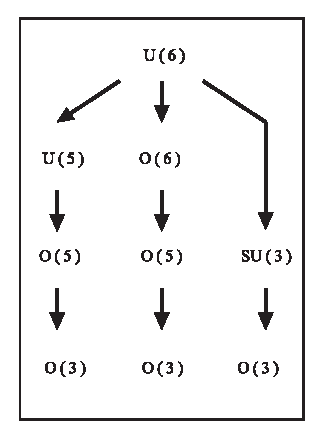
\includegraphics[scale=.65]{figure}
%
% If not, use
%\picplace{5cm}{2cm} % Give the correct figure height and width in cm
%
\caption{If the width of the figure is less than 7.8 cm use the \texttt{sidecapion} command to flush the caption on the left side of the page. If the figure is positioned at the top of the page, align the sidecaption with the top of the figure -- to achieve this you simply need to use the optional argument \texttt{[t]} with the \texttt{sidecaption} command}
\label{fig:1}       % Give a unique label
\end{figure}


\paragraph{Paragraph Heading} %
Instead of simply listing headings of different levels we recommend to let every heading be followed by at least a short passage of text. Furtheron please use the \LaTeX\ automatism for all your cross-references and citations as has already been described in Sect.~\ref{sec:2}.

Please note that the first line of text that follows a heading is not indented, whereas the first lines of all subsequent paragraphs are.

For typesetting numbered lists we recommend to use the \verb|enumerate| environment -- it will automatically render Springer's preferred layout.

\begin{enumerate}
\item{Livelihood and survival mobility are oftentimes coutcomes of uneven socioeconomic development.}
\begin{enumerate}
\item{Livelihood and survival mobility are oftentimes coutcomes of uneven socioeconomic development.}
\item{Livelihood and survival mobility are oftentimes coutcomes of uneven socioeconomic development.}
\end{enumerate}
\item{Livelihood and survival mobility are oftentimes coutcomes of uneven socioeconomic development.}
\end{enumerate}


\subparagraph{Subparagraph Heading} In order to avoid simply listing headings of different levels we recommend to let every heading be followed by at least a short passage of text. Use the \LaTeX\ automatism for all your cross-references and citations as has already been described in Sect.~\ref{sec:2}, see also Fig.~\ref{fig:2}.

Please note that the first line of text that follows a heading is not indented, whereas the first lines of all subsequent paragraphs are.

For unnumbered list we recommend to use the \verb|itemize| environment -- it will automatically render Springer's preferred layout.

\begin{itemize}
\item{Livelihood and survival mobility are oftentimes coutcomes of uneven socioeconomic development, cf. Table~\ref{tab:1}.}
\begin{itemize}
\item{Livelihood and survival mobility are oftentimes coutcomes of uneven socioeconomic development.}
\item{Livelihood and survival mobility are oftentimes coutcomes of uneven socioeconomic development.}
\end{itemize}
\item{Livelihood and survival mobility are oftentimes coutcomes of uneven socioeconomic development.}
\end{itemize}

\begin{figure}[t]
\sidecaption[t]
% Use the relevant command for your figure-insertion program
% to insert the figure file.
% For example, with the option graphics use
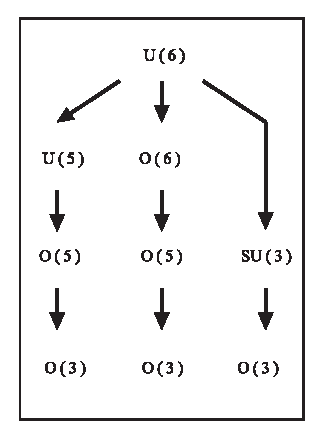
\includegraphics[scale=.65]{figure}
%
% If not, use
%\picplace{5cm}{2cm} % Give the correct figure height and width in cm
%
\caption{Please write your figure caption here}
\label{fig:2}       % Give a unique label
\end{figure}

\runinhead{Run-in Heading Boldface Version} Use the \LaTeX\ automatism for all your cross-references and citations as has already been described in Sect.~\ref{sec:2}.

\subruninhead{Run-in Heading Boldface and Italic Version} Use the \LaTeX\ automatism for all your cross-refer\-ences and citations as has already been described in Sect.~\ref{sec:2}\index{paragraph}.

\subsubruninhead{Run-in Heading Displayed Version} Use the \LaTeX\ automatism for all your cross-refer\-ences and citations as has already been described in Sect.~\ref{sec:2}\index{paragraph}.
% Use the \index{} command to code your index words
%
% For tables use
%
\begin{table}[!t]
\caption{Please write your table caption here}
\label{tab:1}       % Give a unique label
%
% For LaTeX tables use
%
\begin{tabular}{p{2cm}p{2.4cm}p{2cm}p{4.9cm}}
\hline\noalign{\smallskip}
Classes & Subclass & Length & Action Mechanism  \\
\noalign{\smallskip}\svhline\noalign{\smallskip}
Translation & mRNA$^a$  & 22 (19--25) & Translation repression, mRNA cleavage\\
Translation & mRNA cleavage & 21 & mRNA cleavage\\
Translation & mRNA  & 21--22 & mRNA cleavage\\
Translation & mRNA  & 24--26 & Histone and DNA Modification\\
\noalign{\smallskip}\hline\noalign{\smallskip}
\end{tabular}
$^a$ Table foot note (with superscript)
\end{table}
%
\section{Section Heading}
\label{sec:3}
% Always give a unique label
% and use \ref{<label>} for cross-references
% and \cite{<label>} for bibliographic references
% use \sectionmark{}
% to alter or adjust the section heading in the running head
Instead of simply listing headings of different levels we recommend to let every heading be followed by at least a short passage of text. Furtheron please use the \LaTeX\ automatism for all your cross-references and citations as has already been described in Sect.~\ref{sec:2}.

Please note that the first line of text that follows a heading is not indented, whereas the first lines of all subsequent paragraphs are.

If you want to list definitions or the like we recommend to use the Springer-enhanced \verb|description| environment -- it will automatically render Springer's preferred layout.

\begin{description}[Type 1]
\item[Type 1]{That addresses central themes pertainng to migration, health, and disease. In Sect.~\ref{sec:1}, Wilson discusses the role of human migration in infectious disease distributions and patterns.}
\item[Type 2]{That addresses central themes pertainng to migration, health, and disease. In Sect.~\ref{subsec:2}, Wilson discusses the role of human migration in infectious disease distributions and patterns.}
\end{description}

\subsection{Subsection Heading} %
In order to avoid simply listing headings of different levels we recommend to let every heading be followed by at least a short passage of text. Use the \LaTeX\ automatism for all your cross-references and citations citations as has already been described in Sect.~\ref{sec:2}.

Please note that the first line of text that follows a heading is not indented, whereas the first lines of all subsequent paragraphs are.

\begin{svgraybox}
If you want to emphasize complete paragraphs of texts we recommend to use the newly defined Springer class option \verb|graybox| and the newly defined environment \verb|svgraybox|. This will produce a 15 percent screened box 'behind' your text.

If you want to emphasize complete paragraphs of texts we recommend to use the newly defined Springer class option and environment \verb|svgraybox|. This will produce a 15 percent screened box 'behind' your text.
\end{svgraybox}


\subsubsection{Subsubsection Heading}
Instead of simply listing headings of different levels we recommend to let every heading be followed by at least a short passage of text. Furtheron please use the \LaTeX\ automatism for all your cross-references and citations as has already been described in Sect.~\ref{sec:2}.

Please note that the first line of text that follows a heading is not indented, whereas the first lines of all subsequent paragraphs are.

\begin{theorem}
Theorem text goes here.
\end{theorem}
%
% or
%
\begin{definition}
Definition text goes here.
\end{definition}

\begin{proof}
%\smartqed
Proof text goes here.
%\qed
\end{proof}

\paragraph{Paragraph Heading} %
Instead of simply listing headings of different levels we recommend to let every heading be followed by at least a short passage of text. Furtheron please use the \LaTeX\ automatism for all your cross-references and citations as has already been described in Sect.~\ref{sec:2}.

Note that the first line of text that follows a heading is not indented, whereas the first lines of all subsequent paragraphs are.
%
% For built-in environments use
%
\begin{theorem}
Theorem text goes here.
\end{theorem}
%
\begin{definition}
Definition text goes here.
\end{definition}
%
\begin{proof}
%\smartqed
Proof text goes here.
%\qed
\end{proof}
%
%
\begin{trailer}{Trailer Head}
If you want to emphasize complete paragraphs of texts in a \verb|Trailer Head| we recommend to
use  \begin{verbatim}\begin{trailer}{Trailer Head}
...
\end{trailer}\end{verbatim}
\end{trailer}
%
\begin{questype}{Questions}
If you want to emphasize complete paragraphs of texts in an \verb|Questions| we recommend to
use  \begin{verbatim}\begin{questype}{Questions}
...
\end{questype}\end{verbatim}
\end{questype}
%
%
\begin{important}{Important}
If you want to emphasize complete paragraphs of texts in an \verb|Important| we recommend to
use  \begin{verbatim}\begin{important}{Important}
...
\end{important}\end{verbatim}
\end{important}
%
\clearpage
\begin{warning}{Attention}
If you want to emphasize complete paragraphs of texts in an \verb|Attention| we recommend to
use  \begin{verbatim}\begin{warning}{Attention}
...
\end{warning}\end{verbatim}
\end{warning}

\begin{programcode}{Program Code}
If you want to emphasize complete paragraphs of texts in a \verb|Program Code| we recommend to
use

\verb|\begin{programcode}{Program Code}|

\verb|\begin{verbatim}...\end{verbatim}|

\verb|\end{programcode}|

\end{programcode}
%
\begin{tips}{Tips}
If you want to emphasize complete paragraphs of texts in a \verb|Tips| we recommend to
use  \begin{verbatim}\begin{tips}{Tips}
...
\end{tips}\end{verbatim}
\end{tips}
%
%
\begin{overview}{Overview}
If you want to emphasize complete paragraphs of texts in an \verb|Overview| we recommend to
use  \begin{verbatim}\begin{overview}{Overview}
...
\end{overview}\end{verbatim}
\end{overview}
\clearpage
\begin{backgroundinformation}{Background Information}
If you want to emphasize complete paragraphs of texts in a \verb|Background|
\verb|Information| we recommend to
use

\verb|\begin{backgroundinformation}{Background Information}|

\verb|...|

\verb|\end{backgroundinformation}|
\end{backgroundinformation}
\begin{legaltext}{Legal Text}
If you want to emphasize complete paragraphs of texts in a \verb|Legal Text| we recommend to
use  \begin{verbatim}\begin{legaltext}{Legal Text}
...
\end{legaltext}\end{verbatim}
\end{legaltext}
%
\begin{acknowledgement}
If you want to include acknowledgments of assistance and the like at the end of an individual chapter please use the \verb|acknowledgement| environment -- it will automatically render Springer's preferred layout.
\end{acknowledgement}
%
\section*{Appendix}
\addcontentsline{toc}{section}{Appendix}
%
When placed at the end of a chapter or contribution (as opposed to at the end of the book), the numbering of tables, figures, and equations in the appendix section continues on from that in the main text. Hence please \textit{do not} use the \verb|appendix| command when writing an appendix at the end of your chapter or contribution. If there is only one the appendix is designated ``Appendix'', or ``Appendix 1'', or ``Appendix 2'', etc. if there is more than one.

\begin{equation}
a \times b = c
\end{equation}
% Problems or Exercises should be sorted chapterwise
\section*{Problems}
\addcontentsline{toc}{section}{Problems}
%
% Use the following environment.
% Don't forget to label each problem;
% the label is needed for the solutions' environment
\begin{prob}
\label{prob1}
A given problem or Excercise is described here. The
problem is described here. The problem is described here.
\end{prob}

\begin{prob}
\label{prob2}
\textbf{Problem Heading}\\
(a) The first part of the problem is described here.\\
(b) The second part of the problem is described here.
\end{prob}

%%%%%%%%%%%%%%%%%%%%%%%% referenc.tex %%%%%%%%%%%%%%%%%%%%%%%%%%%%%%
% sample references
% %
% Use this file as a template for your own input.
%
%%%%%%%%%%%%%%%%%%%%%%%% Springer-Verlag %%%%%%%%%%%%%%%%%%%%%%%%%%
%
% BibTeX users please use
% \bibliographystyle{}
% \bibliography{}
%
%\biblstarthook{
\section{Styling of References}
In view of the parallel print and (chapter-wise) online publication of your book at \url{www.springerlink.com} it has been decided that -- as a genreral rule --  references should be sorted chapter-wise and placed at the end of the individual chapters. However, upon agreement with your contact at Springer you may list your references in a single seperate chapter at the end of your book. Deactivate the class option \texttt{sectrefs} and the \texttt{thebibliography} environment will be put out as a chapter of its own.\\\indent
References may be \textit{cited} in the text either by number (preferred) or by author/year.\footnote{Make sure that all references from the list are cited in the text. Those not cited should be moved to a separate \textit{Further Reading} section or chapter.} If the citatiion in the text is numbered, the reference list should be arranged in ascending order. If the citation in the text is author/year, the reference list should be \textit{sorted} alphabetically and if there are several works by the same author, the following order should be used:
\begin{enumerate}
\item all works by the author alone, ordered chronologically by year of publication
\item all works by the author with a coauthor, ordered alphabetically by coauthor
\item all works by the author with several coauthors, ordered chronologically by year of publication.
\end{enumerate}
The \textit{styling} of references\footnote{Always use the standard abbreviation of a journal's name according to the ISSN \textit{List of Title Word Abbreviations}, see \url{http://www.issn.org/en/node/344}} depends on the subject of your book:
\begin{itemize}
\item The \textit{two} recommended styles for references in books on \textit{mathematical, physical, statistical and computer sciences} are depicted in ~\cite{science-contrib, science-online, science-mono, science-journal, science-DOI} and ~\cite{phys-online, phys-mono, phys-journal, phys-DOI, phys-contrib}.
\item Examples of the most commonly used reference style in books on \textit{Psychology, Social Sciences} are~\cite{psysoc-mono, psysoc-online,psysoc-journal, psysoc-contrib, psysoc-DOI}.
\item Examples for references in books on \textit{Humanities, Linguistics, Philosophy} are~\cite{humlinphil-journal, humlinphil-contrib, humlinphil-mono, humlinphil-online, humlinphil-DOI}.
\item Examples of the basic Springer style used in publications on a wide range of subjects such as \textit{Computer Science, Economics, Engineering, Geosciences, Life Sciences, Medicine, Biomedicine} are ~\cite{basic-contrib, basic-online, basic-journal, basic-DOI, basic-mono}. 
\end{itemize}
%}

\begin{thebibliography}{99.}%
% and use \bibitem to create references.
%
% Use the following syntax and markup for your references if 
% the subject of your book is from the field 
% "Mathematics, Physics, Statistics, Computer Science"
%
% Contribution 
\bibitem{science-contrib} Broy, M.: Software engineering --- from auxiliary to key technologies. In: Broy, M., Dener, E. (eds.) Software Pioneers, pp. 10-13. Springer, Heidelberg (2002)
%
% Online Document
\bibitem{science-online} Dod, J.: Effective substances. In: The Dictionary of Substances and Their Effects. Royal Society of Chemistry (1999) Available via DIALOG. \\
\url{http://www.rsc.org/dose/title of subordinate document. Cited 15 Jan 1999}
%
% Monograph
\bibitem{science-mono} Geddes, K.O., Czapor, S.R., Labahn, G.: Algorithms for Computer Algebra. Kluwer, Boston (1992) 
%
% Journal article
\bibitem{science-journal} Hamburger, C.: Quasimonotonicity, regularity and duality for nonlinear systems of partial differential equations. Ann. Mat. Pura. Appl. \textbf{169}, 321--354 (1995)
%
% Journal article by DOI
\bibitem{science-DOI} Slifka, M.K., Whitton, J.L.: Clinical implications of dysregulated cytokine production. J. Mol. Med. (2000) doi: 10.1007/s001090000086 
%
%\bigskip

% Use the following (APS) syntax and markup for your references if 
% the subject of your book is from the field 
% "Mathematics, Physics, Statistics, Computer Science"
%
% Online Document
\bibitem{phys-online} J. Dod, in \textit{The Dictionary of Substances and Their Effects}, Royal Society of Chemistry. (Available via DIALOG, 1999), 
\url{http://www.rsc.org/dose/title of subordinate document. Cited 15 Jan 1999}
%
% Monograph
\bibitem{phys-mono} H. Ibach, H. L\"uth, \textit{Solid-State Physics}, 2nd edn. (Springer, New York, 1996), pp. 45-56 
%
% Journal article
\bibitem{phys-journal} S. Preuss, A. Demchuk Jr., M. Stuke, Appl. Phys. A \textbf{61}
%
% Journal article by DOI
\bibitem{phys-DOI} M.K. Slifka, J.L. Whitton, J. Mol. Med., doi: 10.1007/s001090000086
%
% Contribution 
\bibitem{phys-contrib} S.E. Smith, in \textit{Neuromuscular Junction}, ed. by E. Zaimis. Handbook of Experimental Pharmacology, vol 42 (Springer, Heidelberg, 1976), p. 593
%
%\bigskip
%
% Use the following syntax and markup for your references if 
% the subject of your book is from the field 
% "Psychology, Social Sciences"
%
%
% Monograph
\bibitem{psysoc-mono} Calfee, R.~C., \& Valencia, R.~R. (1991). \textit{APA guide to preparing manuscripts for journal publication.} Washington, DC: American Psychological Association.
%
% Online Document
\bibitem{psysoc-online} Dod, J. (1999). Effective substances. In: The dictionary of substances and their effects. Royal Society of Chemistry. Available via DIALOG. \\
\url{http://www.rsc.org/dose/Effective substances.} Cited 15 Jan 1999.
%
% Journal article
\bibitem{psysoc-journal} Harris, M., Karper, E., Stacks, G., Hoffman, D., DeNiro, R., Cruz, P., et al. (2001). Writing labs and the Hollywood connection. \textit{J Film} Writing, 44(3), 213--245.
%
% Contribution 
\bibitem{psysoc-contrib} O'Neil, J.~M., \& Egan, J. (1992). Men's and women's gender role journeys: Metaphor for healing, transition, and transformation. In B.~R. Wainrig (Ed.), \textit{Gender issues across the life cycle} (pp. 107--123). New York: Springer.
%
% Journal article by DOI
\bibitem{psysoc-DOI}Kreger, M., Brindis, C.D., Manuel, D.M., Sassoubre, L. (2007). Lessons learned in systems change initiatives: benchmarks and indicators. \textit{American Journal of Community Psychology}, doi: 10.1007/s10464-007-9108-14.
%
%
% Use the following syntax and markup for your references if 
% the subject of your book is from the field 
% "Humanities, Linguistics, Philosophy"
%
%\bigskip
%
% Journal article
\bibitem{humlinphil-journal} Alber John, Daniel C. O'Connell, and Sabine Kowal. 2002. Personal perspective in TV interviews. \textit{Pragmatics} 12:257--271
%
% Contribution 
\bibitem{humlinphil-contrib} Cameron, Deborah. 1997. Theoretical debates in feminist linguistics: Questions of sex and gender. In \textit{Gender and discourse}, ed. Ruth Wodak, 99--119. London: Sage Publications.
%
% Monograph
\bibitem{humlinphil-mono} Cameron, Deborah. 1985. \textit{Feminism and linguistic theory.} New York: St. Martin's Press.
%
% Online Document
\bibitem{humlinphil-online} Dod, Jake. 1999. Effective substances. In: The dictionary of substances and their effects. Royal Society of Chemistry. Available via DIALOG. \\
http://www.rsc.org/dose/title of subordinate document. Cited 15 Jan 1999
%
% Journal article by DOI
\bibitem{humlinphil-DOI} Suleiman, Camelia, Daniel C. O'Connell, and Sabine Kowal. 2002. `If you and I, if we, in this later day, lose that sacred fire...': Perspective in political interviews. \textit{Journal of Psycholinguistic Research}. doi: 10.1023/A:1015592129296.
%
%
%
%\bigskip
%
%
% Use the following syntax and markup for your references if 
% the subject of your book is from the field 
% "Computer Science, Economics, Engineering, Geosciences, Life Sciences"
%
%
% Contribution 
\bibitem{basic-contrib} Brown B, Aaron M (2001) The politics of nature. In: Smith J (ed) The rise of modern genomics, 3rd edn. Wiley, New York 
%
% Online Document
\bibitem{basic-online} Dod J (1999) Effective Substances. In: The dictionary of substances and their effects. Royal Society of Chemistry. Available via DIALOG. \\
\url{http://www.rsc.org/dose/title of subordinate document. Cited 15 Jan 1999}
%
% Journal article by DOI
\bibitem{basic-DOI} Slifka MK, Whitton JL (2000) Clinical implications of dysregulated cytokine production. J Mol Med, doi: 10.1007/s001090000086
%
% Journal article
\bibitem{basic-journal} Smith J, Jones M Jr, Houghton L et al (1999) Future of health insurance. N Engl J Med 965:325--329
%
% Monograph
\bibitem{basic-mono} South J, Blass B (2001) The future of modern genomics. Blackwell, London 
%
\end{thebibliography}


%%%%%%%%%%%%%%%%%%%%%% appendix.tex %%%%%%%%%%%%%%%%%%%%%%%%%%%%%%%%%
%
% sample appendix
%
% Use this file as a template for your own input.
%
%%%%%%%%%%%%%%%%%%%%%%%% Springer-Verlag %%%%%%%%%%%%%%%%%%%%%%%%%%

\chapter{Chapter Heading}
\label{introA} % Always give a unique label
% use \chaptermark{}
% to alter or adjust the chapter heading in the running head

Use the template \emph{appendix.tex} together with the document class SVMono (monograph-type books) or SVMult (edited books) to style appendix of your book.


\section{Section Heading}
\label{sec:A1}
% Always give a unique label
% and use \ref{<label>} for cross-references
% and \cite{<label>} for bibliographic references
% use \sectionmark{}
% to alter or adjust the section heading in the running head
Instead of simply listing headings of different levels we recommend to let every heading be followed by at least a short passage of text. Further on please use the \LaTeX\ automatism for all your cross-references and citations.


\subsection{Subsection Heading}
\label{sec:A2}
Instead of simply listing headings of different levels we recommend to let every heading be followed by at least a short passage of text. Further on please use the \LaTeX\ automatism for all your cross-references and citations as has already been described in Sect.~\ref{sec:A1}.

For multiline equations we recommend to use the \verb|eqnarray| environment.
\begin{eqnarray}
\vec{a}\times\vec{b}=\vec{c} \nonumber\\
\vec{a}\times\vec{b}=\vec{c}
\label{eq:A01}
\end{eqnarray}

\subsubsection{Subsubsection Heading}
Instead of simply listing headings of different levels we recommend to let every heading be followed by at least a short passage of text. Further on please use the \LaTeX\ automatism for all your cross-references and citations as has already been described in Sect.~\ref{sec:A2}.

Please note that the first line of text that follows a heading is not indented, whereas the first lines of all subsequent paragraphs are.

% For figures use
%
\begin{figure}[t]
\sidecaption[t]
% Use the relevant command for your figure-insertion program
% to insert the figure file.
% For example, with the graphicx style use
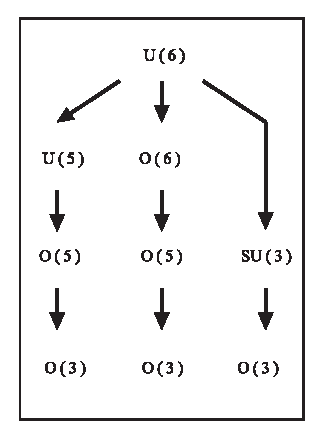
\includegraphics[scale=.65]{figure}
%
% If no graphics program available, insert a blank space i.e. use
%\picplace{5cm}{2cm} % Give the correct figure height and width in cm
%
\caption{Please write your figure caption here}
\label{fig:A1}       % Give a unique label
\end{figure}

% For tables use
%
\begin{table}
\caption{Please write your table caption here}
\label{tab:A1}       % Give a unique label
%
% Follow this input for your own table layout
%
\begin{tabular}{p{2cm}p{2.4cm}p{2cm}p{4.9cm}}
\hline\noalign{\smallskip}
Classes & Subclass & Length & Action Mechanism  \\
\noalign{\smallskip}\hline\noalign{\smallskip}
Translation & mRNA$^a$  & 22 (19--25) & Translation repression, mRNA cleavage\\
Translation & mRNA cleavage & 21 & mRNA cleavage\\
Translation & mRNA  & 21--22 & mRNA cleavage\\
Translation & mRNA  & 24--26 & Histone and DNA Modification\\
\noalign{\smallskip}\hline\noalign{\smallskip}
\end{tabular}
$^a$ Table foot note (with superscript)
\end{table}
%


\backmatter%%%%%%%%%%%%%%%%%%%%%%%%%%%%%%%%%%%%%%%%%%%%%%%%%%%%%%%
%%%%%%%%%%%%%%%%%%%%%%%acronym.tex%%%%%%%%%%%%%%%%%%%%%%%%%%%%%%%%%%%%%%%%%
% sample list of acronyms
%
% Use this file as a template for your own input.
%
%%%%%%%%%%%%%%%%%%%%%%%% Springer Nature%%%%%%%%%%%%%%%%%%%%%%%%%%

\Extrachap{Glossary}


Use the template \emph{glossary.tex} together with the Springer Nature document class SVMono (monograph-type books) or SVMult (edited books) to style your glossary\index{glossary} in the Springer Nature layout.


\runinhead{glossary term} Write here the description of the glossary term. Write here the description of the glossary term. Write here the description of the glossary term.

\runinhead{glossary term} Write here the description of the glossary term. Write here the description of the glossary term. Write here the description of the glossary term.

\runinhead{glossary term} Write here the description of the glossary term. Write here the description of the glossary term. Write here the description of the glossary term.

\runinhead{glossary term} Write here the description of the glossary term. Write here the description of the glossary term. Write here the description of the glossary term.

\runinhead{glossary term} Write here the description of the glossary term. Write here the description of the glossary term. Write here the description of the glossary term.
%
\Extrachap{Solutions}

\section*{Problems of Chapter~\ref{intro}}

\begin{sol}{prob1}
The solution\index{problems}\index{solutions} is revealed here.
\end{sol}


\begin{sol}{prob2}
\textbf{Problem Heading}\\
(a) The solution of first part is revealed here.\\
(b) The solution of second part is revealed here.
\end{sol}


%\printindex

%%%%%%%%%%%%%%%%%%%%%%%%%%%%%%%%%%%%%%%%%%%%%%%%%%%%%%%%%%%%%%%%%%%%%%

\end{document}





